%
% FH Technikum Wien
% !TEX encoding = UTF-8 Unicode
%
% Erstellung von Master- und Bachelorarbeiten an der FH Technikum Wien mit Hilfe von LaTeX und der Klasse TWBOOK
%
% Um ein eigenes Dokument zu erstellen, müssen Sie folgendes ergänzen:
% 1) Mit \documentclass[..] einstellen: Master- oder Bachelorarbeit, Studiengang und Sprache
% 2) Mit \newcommand{\FHTWCitationType}.. Zitierstandard festlegen (wird in der Regel vom Studiengang vorgegeben - bitte erfragen)
% 3) Deckblatt, Kurzfassung, etc. ausfüllen
% 4) und die Arbeit schreiben (die verwendeten Literaturquellen in Literatur.bib eintragen)
%
% Getestet mit TeXstudio mit Zeichenkodierung ISO-8859-1 (=ansinew/latin1) und MikTex unter Windows
% Zu beachten ist, dass die Kodierung der Datei mit der Kodierung des paketes inputenc zusammen passt!
% Die Kodierung der Datei twbook.cls MUSS ANSI betragen!
% Bei der Verwendung von UTF8 muss dnicht nur die Kodierung des Dokuments auf UTF8 gestellt sein, sondern auch die des BibTex-Files!
%
% Bugreports und Feedback bitte per E-Mail an latex@technikum-wien.at
%
% Versionen
% *) V0.7: 9.1.2015, RO: Modeline angepasst und verschoben
% *) V0.6: 10.10.2014, RO: Weitere Anpassung an die UK
% *) V0.5: 8.8.2014, WK: Literaturquellen überarbeitet und angepasst
% *) V0.4: 4.8.2014, WK: Initalversion in SVN eingespielt
%
\documentclass[MSE,Master,english]{twbook}%\documentclass[Bachelor,BMR,ngerman]{twbook}
\usepackage[utf8]{inputenc}
\usepackage[T1]{fontenc}
\usepackage{float}
\usepackage{csquotes}

\newboolean{showImages}
\setboolean{showImages}{true}

\newboolean{showListings} 
\setboolean{showListings}{true}

\newboolean{showTables}
\setboolean{showTables}{true} 

\newboolean{showAppliedMethodsCustomNginxConfSection}
\setboolean{showAppliedMethodsCustomNginxConfSection}{true}

\newboolean{showAppliedMethodsLoadRemoteSettingsSection}
\setboolean{showAppliedMethodsLoadRemoteSettingsSection}{true}

\newboolean{showAppliedMethodsSecondaryEntrypoints}
\setboolean{showAppliedMethodsSecondaryEntrypoints}{true}

\newboolean{showAppliedMethodsTestingQueryReduction}
\setboolean{showAppliedMethodsTestingQueryReduction}{true}

\newboolean{showResultsChapter}
\setboolean{showResultsChapter}{true}

\newboolean{showDiscussionChapter}
\setboolean{showDiscussionChapter}{true}

\newboolean{showConclusionChapter}
\setboolean{showConclusionChapter}{true}

\newboolean{showFutureWorkChapter}
\setboolean{showFutureWorkChapter}{true}

%
% Hier biblatex & Biber konfigurieren; Vergessen Sie nicht, dass Sie biber verwenden müssen um eine Bibliothek zu erzeugen
%
\usepackage[backend=biber, style=numeric]{biblatex}
\usepackage{pgfplots} 
\addbibresource{literature.bib}

%
% Bei Bedarf bitte hier die Syntax-Highlightings anpassen
%
\usepackage{minted}
\makeatletter
% Setzen der Bezeichnungen für das Quellcodeverzeichnis/Abkürzungsverzeichnis in Abhängigkeit von der eingestellten Sprache
\providecommand\listacroname{}
\@ifclasswith{twbook}{english}
{%
    \renewcommand\listoflistingscaption{List of source codes}
    \renewcommand\listacroname{List of Abbreviations}
}{%
    \renewcommand\listoflistingscaption{Quellcodeverzeichnis}
    \renewcommand\listacroname{Abkürzungsverzeichnis}
}
\makeatother

% Die nachfolgenden Pakete stellen sonst nicht benötigte Features zur Verfügung
\usepackage{blindtext}

%
% Einträge für Deckblatt, Kurzfassung, etc.
%
\title{Can GraphQL bring a performance improvement in micro-frontend architectures?}
\author{Florian Mold, BSc}
\studentnumber{11776836}
%\author{Titel Vorname Name, Titel\and{}Titel Vorname Name, Titel}
%\studentnumber{XXXXXXXXXXXXXXX\and{}XXXXXXXXXXXXXXX}
\supervisor{David Leitner, MSc}
%\supervisor[Begutachter]{Titel Vorname Name, Titel}
%\supervisor[Begutachterin]{Titel Vorname Name, Titel}
\secondsupervisor{Gehard Apfelthaler}
%\secondsupervisor[Begutachter]{Titel Vorname Name, Titel}
%\secondsupervisor[Begutachterinnen]{Titel Vorname Name, Titel}
\place{Wien}
\kurzfassung{}
\schlagworte{GraphQL, Micro-frontend, Caching, Backend For Frontend, Apollo Client, Angular React, Webpack}
\outline{}

\keywords{GraphQL, Micro-frontend, Caching, Backend For Frontend, Apollo Client, Angular React, Webpack}
\acknowledgements{Danke an meinen Betreuer David Leitner für die Unterstützung und die vielen hilfreichen Tipps. } 

\begin{document}

\maketitle


\chapter{Introduction}\label{chapter:introduction}
 
The company AGnet has an outdated monolithic system to manage its customers, sales and so on. The technology stack is outdated which is why a migration to a newer technology is necessary. The new architecture should consist of micro-frontends and microservices. Some microservices are already in development, the micro-frontends should be prototyped in the course of this work. Micro-frontends have different problems than traditional frontend-applications. The prototype that is developed should tackle the problems that a distributed architecture brings to the table.
 
This project report is structured in a theoretical part. It is followed by a practical part. In the final chapters the results of the work are presented and discussed. This chapter describes the motivation the hypothesis and state-of-the-art solutions for the project report. Chapter \ref{chapter:applied-methods} covers the methods applied to optimize the number of requests and reduce the network-traffic. The results can be found in Chapter \ref{chapter:results} and the discussion resolving around the result is in Chapter \ref{chapter:discussion}. The final Chapter \ref{chapter:conclusion} concludes the report.

\section{Motivation}

The motivation behind this project report is the creation of a micro-frontend prototype that should replace the old monolithic application within AGnet. The prototype should be more or less equal to the old applications in terms of functionality. The introduction of microservices in the company comes with other problems than a monolithic frontend. For example, all micro-frontends could potentially request the authenticated user. This leads to increased network traffic in comparison to a traditional frontend monotlith.

These problems should be researched and solved through using GraphQL. Many GraphQL clients provide some form of caching. Caching should be used to provide a single caching layer for all micro-frontends to avoid multiple requests to the same resource. GraphQL offers the possibility that the client directly writes the query to the backend. GraphQL provides the ability for the client to write the query directly to the backend. This opens the possibility of removing fields from GraphQL queries that are already in cache. These approaches to improving performance should be evaluated and compared to the naive approach without any optimizations.

\section{Hypothesis}

The first hypothesis focuses on the performance improvement that GraphQL can bring to micro-frontend architectures.

\paragraph{Hypothesis 1} 
A micro-frontend architecture using a shared GraphQL caching layer with partial data can solve the problems of over-fetching and over-requesting inside a distributed architecture. The total number of network-requests and network-traffic can be drastically reduced.\\\\

The second hypothesis focuses on the fact that the creation of a micro-frontend architecture should not depend on a single technology.

\paragraph{Hypothesis 2}
The micro-frontend architecture of the prototype provides enough freedom for an individual choice of technology.\\\\

The result of the work is the proof that GraphQL can solve problems of a micro-frontend architecture. The proof is provided through designing a micro-frontend architecture and writing a shared caching layer.


\chapter{Background}

This chapter will give insights into the most important topics and technologies relevant for this thesis. At the beginning, the 

Afterwards a brief overview of GraphQL is presented. Additional

\section{Micro-Frontend Architecture}

Micro-frontends try to apply the same principles from the microservice architecture to frontend development. Often times a microservice architecture with is developed by several teams has only one frontend application. Therefore, when adding new features a single team can be overwhelmed. Like a microservice architecture, a micro-frontend architecture focuses on developing many small frontend-applications, instead of developing a large software monolith. Each micro-frontend can be developed independently by another team. But a challenge is that the micro-frontend should appear as a single application to the user. Therefore, the different applications have to be integrated, which can be a challenge.

The term micro-frontend should not lead to false conclusions about the size of an application. The size of micro-frontends can vary. It can range from a simple login to a complex single-page application.

Building micro-frontends with the web allows different strategies of integrating the applications. Three different strategies exist to combine multiple micro-frontends into an app-shell. The client-side integration, the server-side integration and the combination of these two strategies and the combination of both strategies.



\subsection{Characteristics}

Micro-frontends tend to follow the same characteristics as microservices.

\subsubsection{Autonomous}

Technically a micro-frontend is a completely independent and runnable application.
The integration of the micro-frontends happens only through the frontend. The different micro-frontends are composed withing an app-shell. The application shell is a separete application that is usually the entry-point for the user to interact with all micro-frontends. The app-shell also provides the layout of the page and defines where the micro-frontends are placed.

\subsubsection{Technology Agnostic}

Just as microservices architectures, micro-frontend architectures can be technology agnostic. The current frontend development landscape offers a lot of JavaScript frameworks to choose from.

\subsubsection{Independently Depoyable}

The autonomy of micro-frontends offer the possibility for independent deployments. A large monolithical micro-frontends is trickier to deploy. There is no need to have communication over multiple teams to deploy the application.


\subsubsection{Small and Easy to Maintain}



\subsubsection{Resilience}



\subsubsection{Resilience}



\subsection{Integration strategies}

\subsubsection{Server-Side Integration}
\subsubsection{Client-Side Integration}

\subsection{Communication}

\subsection{Backend-For-Frontend Pattern}

\section{GraphQL}

The officical documentation states that GraphQL is a query language for APIs and a runtime for fulfilling those queries with your existing data. GraphQL provides a complete and understandable description of the data in your API, gives clients the power to ask for exactly what they need and nothing more, makes it easier to evolve APIs over time, and enables powerful developer tools. GraphQL is implemented in many languages and frameworks. It has a large ecosystem of libraries and tools.

\subsection{Origins and history}

GraphQL was initially developed at Facebook in 2012. In 2015 the project was made open-source and available to the public. The motivation behind the initial development of GraphQL was the limited flexibility of available API technologies like REST.

\subsection{Apollo Server and Client}

GraphQL is a query language and follows specific rules. The development of a GraphQL server and client is up to the application developer. Facebook has developed their own implementation of a GraphQL server and client. The server is called GraphQL.js and the client is called Relay.

Apollo 

Apollo Client is m

\subsubsection{How does the in-memory cache work?}

This section describes how the cache in apollo-client works. By default all GraphQL requests made with \textbf{ApolloClient} are cached inside the browsers memory. This enables Apollo Client to respond almost immediately to queries for already-cached data, without even sending a network request. This is needed, to ensure to reduce round-trips to the server in subsequent requests of the same query, because the requested data can be served from the cache. The caching mechanism reduces the load of the server, but introduces issues with cache management. \textbf{ApolloClient} includes a caching mechanism called ApolloCache and the propretary implementation called \textbf{InMemoryCache}. There are several Open-Source alternatives, that implement the \textbf{ApolloCache} interface.

\ifshowImages
\begin{figure}[!htbp]
\centering
\includegraphics[width=0.6\linewidth]{images/background/apollo/apollo-client-basic-cache.jpeg}
\caption{All requests made during the measurement of the first approach}\label{figure:background:user-query-first-time}
\end{figure}
\fi

The flow of the cache, when the query \textbf{user} is executed the first time is shown in figure \ref{figure:background:user-query-first-time}.


\ifshowImages
\begin{figure}[!htbp]
\centering
\includegraphics[width=0.6\linewidth]{images/background/apollo/apollo-client-basic-cache-warm.jpeg}
\caption{All requests made during the measurement of the first approach}\label{figure:background:user-query-second-time}
\end{figure}
\fi

When the query is executed later with the same parameters, the flow looks like in figure \ref{figure:background:user-query-second-time}.

In order to correctly understand cache updates, it is important to understand the structure of the cache. The structure of the \textbf{InMemoryCache} is a simple normalized object. When the cache is empty, it is just an empty object. When the following query is requested from the server and the response is stored in the cache, the cache will look like this:

\ifshowListings
\begin{listing}[H]
\begin{minted}{typescript}
query {
  users {
    id
    username
    email
  }
}
\end{minted}
\caption{An example of a query}\label{code:background:query-user-cache}
\end{listing}
\fi

And the server responds with the following result. The \textbf{\_\_typename} property is automatically appended to the query by the \textbf{ApolloClient}.

\ifshowListings
\begin{listing}[H]
\begin{minted}{typescript}
{
  users: [
    {
      __typename: 'User',
      id: '36bad921-8fcf-4f33-9f29-0d3cd70205c8',
      username: 'Florian',
      email: 'florian@test.io'
    }, 
    {
      __typename: 'User',
      id: 'a2096556-9a4e-4994-9de8-86c9e85ed6a1',
      username: 'Daniel',
      email: 'daniel@test.io'
    }
  ]
}
\end{minted}
\caption{The result of the GraphQL query from listing \ref{code:background:query-user-cache}}\label{code:background:query-user-response-result}
\end{listing}
\fi

The \textbf{ApolloClient} will update the cache so that it looks like this.

\ifshowListings
\begin{listing}[H]
\begin{minted}{typescript}
{
  ROOT_QUERY: {
    __typename: 'Query',
    users: [
      { __ref: 'User:36bad921-8fcf-4f33-9f29-0d3cd70205c8', },
      { __ref: 'User:a2096556-9a4e-4994-9de8-86c9e85ed6a1', },
    ],
  },
  'User:36bad921-8fcf-4f33-9f29-0d3cd70205c8': {
    __typeName: 'User',
    id: '36bad921-8fcf-4f33-9f29-0d3cd70205c8',
    username: 'Florian',
    email: 'florian@test.io',
  },
  'User:a2096556-9a4e-4994-9de8-86c9e85ed6a1': {
    __typeName: 'User',
    id: 'a2096556-9a4e-4994-9de8-86c9e85ed6a1',
    username: 'Daniel',
    email: 'daniel@test.io',
  }
}
\end{minted}
\caption{The data inside the cache with the response from listing \ref{code:background:query-user-response-result}}\label{code:background:query-user-cache-representation}
\end{listing}
\fi

Let's describe how the response from the server is transformed into the representation from the cache seen in listing \ref{code:background:query-user-cache-representation}. The cache object contains a key \textbf{ROOT\_QUERY}. This element contains the name of the queries that were executed and the results from all queries. The query \textbf{allUsers} was fetched, therefore the \textbf{ROOT\_Query} contains a field with the name \textbf{users}. The listing \ref{code:background:query-user-cache-representation} shows that the content of the \textbf{ApolloClient} is clearly different from the servers response. Instead of the user-information every array item consists of an object with a \textbf{\_\_ref} key. The value of the key is simply the \textbf{\_\_typename} and \textbf{id} of the user concatenated. The data from the response has been normalised and added to the cache object. Next to the \textbf{ROOT\_QUERY} element, the actual user-information is stored. Each has the same key as the \textbf{\_\_ref} from the \textbf{ROOT\_QUERY}. 

The same principle applies to arbitrary deep queries. The following query produces:

\ifshowListings
\begin{listing}[H]
\begin{minted}{typescript}
query {
  allUsers {
    id
    username
    Title {
      id
      name
    }
  }
}
\end{minted}
\caption{An example of a query}\label{code:background:nested-query-user-cache}
\end{listing}
\fi

And the server responds with the following result. The \textbf{\_\_typename} property is automatically appended to the query by the \textbf{ApolloClient}.

\ifshowListings
\begin{listing}[H]
\begin{minted}{typescript}
{
  users: [
    {
      __typename: 'User',
      id: '36bad921-8fcf-4f33-9f29-0d3cd70205c8',
      username: 'Florian',
      title: {
        __typename: 'Title',
        id: '2adb1120-d911-4196-ab1b-d5043cc7a00a',
        name: 'BSc.'
      }
    }, 
    {
      __typename: 'User',
      id: 'a2096556-9a4e-4994-9de8-86c9e85ed6a1',
      username: 'Daniel',
      title: {
        __typename: 'Title',
        id: '2adb1120-d911-4196-ab1b-d5043cc7a00a',
        name: 'BSc.'
      }
    }
  ]
}
\end{minted}
\caption{The result of the GraphQL query from listing \ref{code:background:nested-query-user-cache}}\label{code:background:nested-query-user-response-result}
\end{listing}
\fi

\ifshowListings
\begin{listing}[H]
\begin{minted}{typescript}
{
  ROOT_QUERY: {
    __typename: 'Query',
    users: [
      { __ref: 'User:36bad921-8fcf-4f33-9f29-0d3cd70205c8', },
      { __ref: 'User:a2096556-9a4e-4994-9de8-86c9e85ed6a1', },
    ],
  },
  'User:36bad921-8fcf-4f33-9f29-0d3cd70205c8': {
    __typeName: 'User',
    id: '36bad921-8fcf-4f33-9f29-0d3cd70205c8',
    username: 'Florian',
    Title: {
      __ref: 'Title:2adb1120-d911-4196-ab1b-d5043cc7a00a',
    },
  },
  'User:a2096556-9a4e-4994-9de8-86c9e85ed6a1': {
    __typeName: 'User',
    id: 'a2096556-9a4e-4994-9de8-86c9e85ed6a1',
    username: 'Daniel',
    Title: {
      __ref: 'Title:2adb1120-d911-4196-ab1b-d5043cc7a00a',
    },
  }
  'Title:2adb1120-d911-4196-ab1b-d5043cc7a00a': {
    __typeName: 'Address',
    id: '2adb1120-d911-4196-ab1b-d5043cc7a00a',
    name: 'BSc.',
  },
}
\end{minted}
\caption{The data inside the cache with the response from listing \ref{code:background:nested-query-user-response-result}}\label{code:background:nested-query-user-cache-representation}
\end{listing}
\fi

The \textbf{ROOT\_QUERY} is exactly the same as with the query before. Each user contains a reference to a title. Both users have the same title, therefore the server returned duplicate data. But the cache normalisation causes the title to be only present once in the cache.

This behaviour is very helpful, because when a cache item is updated, the entire cache object doesn't have to be traversed in search for the instance that has been changed. Only a single item has to updated.

The cache normalisation works when the query contains either a \textbf{\_id} or \textbf{id} field. Without an id the object can't be normalized. Here is an example:

\ifshowListings
\begin{listing}[H]
\begin{minted}{typescript}
query {
  allUsers {
    id
    username
    Title {
      name
    }
  }
}
\end{minted}
\caption{An example of a query}\label{code:background:no-id-query-user-cache}
\end{listing}
\fi

The response: 

\ifshowListings
\begin{listing}[H]
\begin{minted}{typescript}
{
  users: [
    {
      __typename: 'User',
      id: '36bad921-8fcf-4f33-9f29-0d3cd70205c8',
      username: 'Florian',
      title: {
        __typename: 'Title',
        name: 'BSc.'
      }
    }, 
    {
      __typename: 'User',
      id: 'a2096556-9a4e-4994-9de8-86c9e85ed6a1',
      username: 'Daniel',
      title: {
        __typename: 'Title',
        name: 'BSc.'
      }
    }
  ]
}
\end{minted}
\caption{The result of the GraphQL query from listing \ref{code:background:no-id-query-user-cache}}\label{code:background:no-id-query-user-response-result}
\end{listing}
\fi

And the cache looks like the following:

\ifshowListings
\begin{listing}[H]
\begin{minted}{typescript}
{
  ROOT_QUERY: {
    __typename: 'Query',
    users: [
      { __ref: 'User:36bad921-8fcf-4f33-9f29-0d3cd70205c8', },
      { __ref: 'User:a2096556-9a4e-4994-9de8-86c9e85ed6a1', },
    ],
  },
  'User:36bad921-8fcf-4f33-9f29-0d3cd70205c8': {
    __typeName: 'User',
    id: '36bad921-8fcf-4f33-9f29-0d3cd70205c8',
    username: 'Florian',
    Title: {
      name: 'BSc.',
    },
  },
  'User:a2096556-9a4e-4994-9de8-86c9e85ed6a1': {
    __typeName: 'User',
    id: 'a2096556-9a4e-4994-9de8-86c9e85ed6a1',
    username: 'Daniel',
    Title: {
      name: 'BSc.',
    },
  }
}
\end{minted}
\caption{The data inside the cache with the response from listing \ref{code:background:no-id-query-user-response-result}}\label{code:background:no-id-query-user-cache-representation}
\end{listing}
\fi

This should be avoided. If data of an unnormalised object has to be updated every occurence of the item in the cache has to be updated manually. You must also never request the same thing sometimes with an id and sometimes without, because \textbf{ApolloClient} will throw an error when trying to update the cache after such a query.


The Apollo Client's cache stores the data a flat lookup table of objects that reference eachother. \cite{misc:-:apollo-cache-overview}

Whenever the Apollo Client receives the response data of a query it does the following. a

\begin{enumerate}
  \item \textbf{Identify objects}:
  \item \textbf{Generate cache IDs}:
  \item \textbf{Replace object fields with references}:
  \item \textbf{Store normalized objects}:
\end{enumerate}

\chapter{Applied Methods}\label{chapter:applied-methods}

This chapter documents how the prototypical micro-frontend architecture was built step by step—the first section centers around identifying bounded contexts and deriving the micro-frontends from them. The following section is about the prototypical implementation of the micro-frontend architecture. After implementing the architecture, the communication patterns between the micro-frontends were analyzed and implemented. The next section centers around developing a shared caching layer. The last section focuses on a mechanism to remove fields from a GraphQL query by utilizing the Apollo Client's in-memory cache. This chapter ends by showing how query reduction works in practice.

\section{Identification of micro-frontends}\label{section:applied-methods:identification-micro-frontends}

The first step before starting to implement the micro-frontend architecture was to identify the parts of the legacy application that should be extracted into microservices and micro-frontends. The application is a large software monolith with a single database. In collaboration with the product owner, parts of the legacy application were identified as candidates for micro-frontends. 

The user interface of the old implementation is also one large application.

\bigskip

\noindent The complete legacy application can't be prototyped in the course of this master-thesis, therefore the three most important bounded contexts were identified. The bounded contexts are the following:

\begin{itemize}
  \item User
  \item Sales
  \item Contact
  \item Dashboard
\end{itemize}

\section{Implementation of a prototypical micro-frontend architecture}

The first step was to implement a prototypical micro-frontend architecture that fits my companies needs. Runtime integration was chosen to take the most advantages of micro front-ends. To implement the runtime

The micro-frontend architecture that powers the prototype was developed using Webpack's Module Federation. The prototype contains a shell-application that loads all other micro-frontends. The architecture is divided into 9 widgets that display only simple data and 3 complex single-page applications.

The main part of the implementation is written in Angular. One micro-frontend was implemented with the frontend-framework React to show that the findings of this project are technology agnostic.

I implemented one micro-frontend in React to show that the architecture is technology agnostic and if it can access the shared Apollo caching layer. For loading and rendering the React micro-frontend inside the host, I had to implement an adapter inside the shell-application. This adapter renders the React application inside a HTMLElement. It also provides the necessary configuration like the instance of the Apollo cache as context to the application.

Every micro-frontend is a complete Angular application that offers all of the features that Angular offers.

A rough overview of the architecture is shown in figure \ref{figure:methods:ui-dashboard-architecture}. The icons inside the squares represent the technology used.

\ifshowImages
\begin{figure}[H]
\centering
\includegraphics[width=0.8\linewidth]{images/ui-dashboard-architecture.jpeg}
\caption{Architecture of the micro-frontend prototype.}\label{figure:methods:ui-dashboard-architecture}
\end{figure}
\fi

The functionality of the micro-frontends is encapsulated in modules that can be used by the shell application. Each icon of Angular and React represents such a module, as shown in figure \ref{figure:methods:ui-dashboard-architecture}. These modules can be used when the application is running in standalone mode, and the modules can be made accessible to the shell application via module federation.

How a module can be exposed to be consumed by a remote application is shown in the listing \ref{code:methods:module-federation-config-expose}.

\ifshowListings
\begin{listing}[H]
\begin{minted}{typescript}
module.exports = {
  name: 'contact',
  exposes: {
    './Module': 'apps/contact/src/app/remote-entry/entry.module.ts',
  },
};
\end{minted}
\caption{Module Federation config to expose an Angular module to be consumed.}\label{code:methods:module-federation-config-expose}
\end{listing}
\fi

The host can configure its Module Federation to to be able to consume the entry.module.ts from the contact micro-frontend. The configuration can be seen in the listing \ref{code:methods:module-federation-config-consume}.

\ifshowListings
\begin{listing}[H]
\begin{minted}{typescript}
module.exports = {
  name: 'host',
  remotes: {
    contact: 'contact@http://localhost:4202/remoteEntry.js'
  },
};
\end{minted}
\caption{Module Federation config that consumes an Angular module from a remote location.}\label{code:methods:module-federation-config-consume}
\end{listing}
\fi

Inside the host application the remote module from the contact application can be easily referenced and routed to. The configuration of the route can be seen in listing \ref{code:methods:angular-route-to-remote-module}

\ifshowListings
\begin{listing}[H]
\begin{minted}{typescript}
const routes: Routes = [
  {
    path: 'contact',
    loadChildren: () =>
    loadRemoteModule(
      'contact',
      './Module'
    ).then((m) => m.UiContactRemoteEntryModule),
  },
  ...
]
\end{minted}
\caption{Route to the exposed remote-module from the contact application}\label{code:methods:angular-route-to-remote-module}
\end{listing}
\fi


\subsection{Module Federation}

\subsection{Integrating react micro-frontend}

\subsection{Backend for frontend architecture}
\section{Communication from the shell- to the remote-application}\label{section:methods:communication-shell-remote}

To solve the problem of building a common caching layer, some form of communication between the shell and remote application had to be implemented. To ensure that the micro-frontends remain independent of each other, it should be avoided that they communicate directly with each other.

Angular provides a great tool for this use case, namely dependency injection. The shell application can provide services that can later be injected by the remote applications. This is very handy because the micro frontend can provide the same services as the shell application in standalone mode. Therefore, the remote module can be easily used within the remote and shell application.

For example i implemented a layout-service that takes advantage of dependency injection.

\ifshowImages
\begin{figure}[H]
\centering
\includegraphics[width=1\linewidth]{images/prototype-screenshots/contact-header.png}
\caption{Beispiel für die Beschriftung eines Buchrückens.}
\end{figure}
\fi

\ifshowImages
\begin{figure}[H]
\centering
\includegraphics[width=1\linewidth]{images/prototype-screenshots/host-contact-header.png}
\caption{Beispiel für die Beschriftung eines Buchrückens.}
\end{figure}
\fi

\section{Shared caching layer between the micro-frontends}

With the knowledge from the previous section \ref{section:methods:communication-shell-remote} a shared caching layer was implemented. Apollo GraphQL was chosen as GraphQL client for this prototype. It offers the most support for various frameworks and has a large community. The shell application can provide the instance of the GraphQL cache, which the micro-frontends can inject and use, when setting up their client, as seen in figure \ref{code:methods:graphql-client-cache-provider}. When running the micro-frontend in standalone mode, this provider has to be used inside the native application of the micro-frontend.

For example the contact-application provides this object seen in listing \ref{code:methods:graphql-client-cache-provider} in its providers-array inside the core.module.ts. The host-application has the exactly same configuration inside its core.module.ts.

\ifshowListings
\begin{listing}[H]
\begin{minted}{typescript}
@NgModule({
  providers: [
    {
      provide: UI_GRAPHQL_CLIENT_CACHE,
      useValue: new InMemoryCache(),
    },
  ],
})
export class UiContactCoreModule {}
\end{minted}
\caption{Provide the instance of the cache to dependency injection.}\label{code:methods:graphql-client-cache-provider}
\end{listing}
\fi

UI\_GRAPHQL\_CLIENT\_CACHE is an Angular Injection-token that can be used to provide injectable objects that can be used with dependency injection. (TODO: Injection token link)

These provider must only be set inside the providers of the core.module.ts that the native application provides. Otherwise the remote-module would have their own instances of the GraphQL cache and the shared caching-layer would not work.

Every micro-frontend can have their own instance of a GraphQL client. Only the GraphQL cache is shared between the different applications. Therefore, in theory, it is also possible that every micro-frontend consumes a different GraphQL API.

\ifshowListings
\begin{listing}[H]
\begin{minted}{typescript}
 @NgModule({
   providers: [
     {
       provide: UI_GRAPHQL_CLIENT_OPTIONS_CONFIG,
       useValue: {
         shareCache: true,
         persistCache: false,
         useTypePolicies: true,
         typePolicies: UI_CONTACT_APP_TYPE_POLICIES,
       } as UiGraphQLClientOptionsConfig,
     },
   ],
 })
 export class UiContactRemoteCoreModule {}
\end{minted}
\caption{Extra configuration TODO}\label{code:methods:graphql-client-extra-configuration-options}
\end{listing}
\fi

To make it simple for the micro-frontends to use GraphQL, a function was written that creates the GraphQL client, seen in listing \ref{code:methods:graphql-client-creation}.

\ifshowListings
\begin{listing}[H]
\begin{minted}{typescript}
UiGraphQLClientOptionsModule.withConfig('contact-remote-app', {
  provideGraphQLClientOptions: true,
}),
\end{minted}
\caption{Provide the instance of the cache as injectable.}\label{code:methods:graphql-client-creation}
\end{listing}
\fi

The first parameter of the function is a unique name for the GraphQL client instance. The unique name is mostly used for logging purposes. The second parameter is a configuration object whose options can be configured that no client is created.

For example the GraphQL client could be already provided inside the core-module of the shell-application and the remote-application injects that instance of the GraphQL client. These configuration options were largely added to test the shared caching layer with different options.

The final architecture follows the approach that each micro-frontend has a separate GraphQL client and a shared cache. This allows for the most flexibility as the GraphQL client can be configured individually by each micro frontend.


My prototype creates 12 GraphQL clients, if every remote-application is loaded.

\begin{enumerate}
  \item host-native-app-graphql-client
  \item contact-remote-app-graphql-client
  \item sales-remote-app-graphql-client
  \item user-remote-app-graphql-client
  \item address-remote-widget-graphql-client
  \item contact-list-remote-widget-graphql-client
  \item contact-remote-widget-graphql-client
  \item contract-remote-widget-graphql-client
  \item invoice-remote-widget-graphql-client
  \item person-remote-widget-graphql-client
  \item sales-remote-widget-graphql-client
  \item user-remote-widget-graphql-client
\end{enumerate}


\section{Built a mechanism that reduces the size of queries}\label{section:applied-methods:query-reduction}

After implementing the shared caching layer, the next step was to improve the performance of the micro-frontends by optimizing the use of the cache. The size of the network requests can be reduced by removing parts of a query that are already inside the cache. The theory behind removing fields from the query was already explained in section \ref{subsection:background:graphql:query-reduction}. The Apollo Client does not provide such a functionality out of the box, but the feature is requested in Apollo's Github Repository by many users. The section \ref{subsubsection:background:graphql:apollo-server-client:in-memory-cache-working} explains how the \texttt{InMemoryCache} cache of Apollo Client works in more detail. Briefly summarized the caching works with the name and the parameters of a GraphQL query. For example, if a query is executed against the GraphQL \ac{API}, the results of the query are cached. If the same query with the same fields is executed again with the same parameters, the results are fetched from the Apollo Client cache. If the query fetches an additional field, which is not inside the cache, the complete query is sent to the GraphQL \ac{API}. Only if the queried fields are completely identical, the data from the cache is used. Consequently, identical queries that fetch different fields are always fetched from the server.

\bigskip

\noindent Consider listing \ref{code:applied-methods:compare-allusers-user-query}, where the left query fetches all users, and the right query fetches a user by its id. Both queries fetch the same data type and the same fields, but they are fundamentally different queries. They have different names and different parameters. Both queries are sent to the GraphQL \ac{API}. The right query could be omitted if the user with the given id is fetched from the cache. If the left query is executed before the right query, the data to resolve the right query could be completely taken from the cache.

\ifshowListings
\begin{listing}[H]
\begin{minted}{typescript}
query allUsers {                        query user(id: ID!) {
  allUsers {                              user(id: \$id) {
    id                                      id
    username                                username
    email                                   email
    firstName                               firstName
    secondName                              secondName
  }                                       }
}                                      }
\end{minted}
\caption{Comparison between the \texttt{allUsers} and \texttt{User} query.}\label{code:applied-methods:compare-allusers-user-query}
\end{listing}
\fi

\noindent Apollo offers a solution to tackle this problem. The application might have a detail view and a list view that both query the same data like in listing \ref{code:applied-methods:compare-allusers-user-query}. The data for the \texttt{user} query might be already in the cache, but the Apollo Client does not know that. Therefore, the lookup of the cache can be configured, so that the Apollo Client knows where to look for the data. To better understand the cache redirection, a basic understanding of type policies is needed, which were described in more detail in section \ref{subsubsection:background:graphql:apollo-server-client:type-policies}.

\bigskip

\noindent To inform the Apollo Client where to look for the cached \texttt{User} object, a field policy \texttt{read} function must be written for the \texttt{user} query. Just like the \texttt{firstName} being a field of the \texttt{User} type is the \texttt{user}-query a field of the root query. This hierarchy resembles the structure of the GraphQL Schema, where the queries have to be defined inside the \texttt{Query} type. Listing \ref{code:applied-methods:query-reduction:graphql-schema} shows an excerpt from the GraphQL schema. All queries that can be executed by a client, are listed inside the \texttt{Query} type.

\ifshowListings
\begin{listing}[H]
\begin{minted}{typescript}
type Query {
  user(id: ID!): User
  allUsers(page: Int, perPage: Int): [User]
  ...
}

type User {
  id: ID!
  firstName: String!
  secondName: String!
  ...
}
\end{minted}
\caption{An excerpt from the GraphQL schema.}\label{code:applied-methods:query-reduction:graphql-schema}
\end{listing}
\fi


\noindent Listing \ref{code:applied-methods:query-reduction:user-cache-redirect} shows the \texttt{read} field policy for the \texttt{User}. Like in the GraphQL schema from listing \ref{code:applied-methods:query-reduction:graphql-schema}, the \texttt{user} query is a field of the root query. Therefore, every time the client queries the \texttt{user} query, the read function is executed. The \texttt{toReference} function is used to a cache reference for a \texttt{User} type. The reference is generated based on its \texttt{\_\_typename} and \texttt{id}, as explained in section \ref{subsubsection:background:graphql:apollo-server-client:data-normalization}. Apollo uses the result of \texttt{toReference} to look up the object in its cache and return it if it is present. If the object is not present in the cache, the query is sent to the GraphQL \ac{API}.

\ifshowListings
\begin{listing}[H]
\begin{minted}{typescript}
new ApolloClient({
  cache: new InMemoryCache({ typePolicies: { Query: { fields: {
    User: {
      read(_, { args, toReference }): {
        return toReference({ __typename: 'User', id: args.id });
      }
    }
  }}}})
});
\end{minted}
\caption{Writing a cache-redirect for the User-type.}\label{code:applied-methods:query-reduction:user-cache-redirect}
\end{listing}
\fi

\noindent Using cache redirects to reduce the amount of network requests works, but all of the query's requested fields must be already present in the cache. If the \texttt{user} query fetches any field that the \texttt{allUsers} query did not, Apollo Client considers the cache hit to be incomplete and the query is executed over the network. That a detail view and a list view are perfectly identical is very rare in applications. Therefore this approach can't be used to reduce the size of network requests effectively. And the approach is very verbose because a redirect has to be written for every data type. The approach does not scale, as the same type-policies would have to be written and registered for every micro-frontend.

\bigskip

\noindent The open source project \href{https://github.com/appmotion/apollo-augmented-hooks}{apollo-augmented-hooks} on GitHub provides drop-in replacements for Apollo's GraphQL query methods. It provides the functionality to remove fields from a query that are already in the cache. However, the big problem is that the project was developed specifically for React's Apollo Client. The dependencies were outdated and the latest release of the library was in 2021. To test the library an older version of Apollo Client was used. The dependency offered the functionality to remove fields that already exist in the cache from a previous GraphQL query. To use the functionality of the library inside the prototypical micro-frontend architecture, the Apollo-augmented-hooks dependency was forked. The first step was to update the dependencies to make it work with the latest version of Apollo Client. The problem with the old implementation is that it just supports React's Apollo Client with its hooks. The core functionality of the library was extracted and an adapter for React and Angular was written utilizing the functionality. The functions have the same \ac{API} as Apollo's original methods, therefore the migration is very easy. The functionality of the library was rewritten with \ac{TS} and some additional features were added, that utilize the cache even more. The implementation is detailed even further in the section \ref{subsection:applied-methods:query-reduction:how-does-the-library-work}.

\ifshowAppliedMethodsTestingQueryReduction
  \subsection{Testing layer}\label{subsection:applied-methods:query-reduction:testing-query-reduction}

The interface seen in Listing \ref{code:applied-methods:query-reduction:graphql-client} is an abstraction for Apollo Client's functionality. The interface was created to allow a comparison between the default Apollo Client behavior and the improved behavior through query reduction. The \texttt{watchQuery} and \texttt{mutate} functions have the same \ac{API} as Apollo Client's original \texttt{watchQuery} and \texttt{mutate} functions. The classes \texttt{ReduceGraphQLClientImpl} and \texttt{GraphQLClientImpl} implement the \texttt{GraphQLClient} interface. The \texttt{ReduceGraphQLClientImpl} uses query reduction functionality, while \texttt{GraphQLClientImpl} utilizes the original Apollo Client functionality. A feature flag is used to determine which implementation is used during runtime.

\ifshowListings
\begin{listing}[H]
\begin{minted}{typescript}
interface GraphQLClient {
  watchQuery<TData, TVariables>(
    options: WatchQueryOptions<TData, TVariables>
  ): Observable<QueryResult<TData>>;

  mutate<TData, TVariables>(
    options: MutationOptions<TData, TVariables>
  ): Observable<MutationResult<TData>>;
}
\end{minted}
\caption{The abstract base class for the Apollo Client.}\label{code:applied-methods:query-reduction:graphql-client}
\end{listing}
\fi

\noindent The feature flag is implemented as an injection token that can be provided within the micro frontends. The injection token \texttt{REDUCE\_QUERY\_OPTIONS} specifies whether \texttt{ReduceGraphQLClientImpl} or \texttt{GraphQLClientImpl} is initialized. The usage of the injection token is shown in the Listing \ref{code:applied-methods:query-reduction:switch-between-apollo-client-and-query-reduction}. The \texttt{ReduceGraphQLClientImpl} is used when the \texttt{reduceQueries} property is set to \texttt{true}, otherwise, the \texttt{GraphQLClientImpl} is initialized.

\ifshowListings
\begin{listing}[H]
\begin{minted}{typescript}
const REDUCE_QUERY_OPTIONS = 
  new InjectionToken<ReduceQueryOptions>('reduce-query-options');

@NgModule({
  providers: [{
    provide: REDUCE_QUERY_OPTIONS,
    useValue: { reduceQueries: true },
  }]
})
class ContactCoreModule {}
\end{minted}
\caption{Specify which \texttt{GraphQLClient} implementation should be used.}\label{code:applied-methods:query-reduction:switch-between-apollo-client-and-query-reduction}
\end{listing}
\fi


\fi

\subsection{Query reduction mechanism}\label{subsection:applied-methods:query-reduction:how-does-the-library-work}

This section briefly describes how the query reduction functionality removes fields from the query using the \texttt{InMemoryCache}. Apollo Client allows specifying multiple configuration options when trying to fetch a query from a GraphQL \ac{API}. The three most important options are \texttt{variables}, \texttt{query}, and \texttt{fetchPolicy}. The \texttt{query} specifies the GraphQL query, and the \texttt{variables} are the variables for the query. The typical structure of a GraphQL query inside the micro-frontend architecture is shown in Listing \ref{code:applied-methods:query-reduction:executing-graphql-query}. The query fetches the user's details with the given \texttt{id}. The default fetch policy of a query is \texttt{cache-first}.  

\ifshowListings
\begin{listing}[H]
\begin{minted}{typescript}
this.graphQLClient.watchQuery({
  variables: { id: '36bad921-8fcf-4f33-9f29-0d3cd70205c8' },
  query: USER_BY_ID_QUERY,
  fetchPolicy: 'cache-first',
});
\end{minted}
\caption{Defining and running a GraphQL query with Apollo Client.}\label{code:applied-methods:query-reduction:executing-graphql-query}
\end{listing}
\fi

\subsubsection{Analysis of the feasibility of reducing queries}

The fetch policy lets the client specify how data is stored and retrieved from the cache. The Apollo Client offers several fetch policies that customize how the client retrieves data from the cache. The five available fetch policies are: \cite{misc:-:applied-methods:query-reduction:apollo-client:queries}

\begin{itemize}
  \item \textbf{cache-first (default)}: This fetch policy instructs the Apollo Client first to check the local cache for the query result. If the data is present in the cache, it is returned immediately. Otherwise, Apollo Client will execute the query and fetch the result from the server, which will then be cached.
  \item \textbf{cache-and-network}: This fetch policy combines the cache-first and network-only policies. Apollo Client first checks the cache for the query result and returns it immediately if it is present. Then, a network request is made to fetch the most up-to-date data, which is then used to update the cache. This fetch policy is a good option for displaying data that gets updated frequently.
  \item \textbf{cache-only}: This fetch policy tells Apollo Client only to check the cache for the query result. If the result is present in the cache, it is returned immediately.
  \item \textbf{network-only}: This fetch policy instructs Apollo Client to skip the cache entirely and always fetch the query result from the server.
  \item \textbf{no-cache}: This fetch policy skips the cache entirely and always fetches the query result from the server. Unlike network-only, the result is not cached.
\end{itemize}

\noindent The first step of the function is whether the fetch policy allows the query to be reduced. Suppose the query is executed with one of the following cache policies: \texttt{cache-only}, \texttt{network-only}, and \texttt{no-cache}; reducing the query is counterproductive. With \texttt{network-only}, the latest data should be fetched from the GraphQL \ac{API}. The \texttt{cache-only} policy only targets the cache; therefore, no reduction is necessary. The \texttt{no-cache} policy bypasses the cache and requests data from the GraphQL \ac{API}. Another feature of Apollo Client is polling. Polling in Apollo Client is a technique used to fetch a query's data at a specified interval periodically, and it allows a near-real-time synchronization with the server. To enable polling for a query, pass a \texttt{pollInterval} (ms) configuration option to the \texttt{watchQuery} method. Removing fields from a query that uses polling does not make sense either because real-time data should be rendered. The following sections describe the steps needed to reduce the query. The micro-frontend architecture uses the cache-first strategy for every query, as it is the only fetch policy that can omit network requests.

\subsubsection{Identify the key fields of every GraphQL type}

The first step is identifying the key fields of the types inside the schema. The contents of the \texttt{InMemoryCache} can be extracted using the \texttt{cache.extract()} function. This function returns an object with all the contents of the cache. The key fields can be read from the configuration of the cache. The implementation returns an object where the type name is the key and the key fields are the value. The \texttt{InMemoryCache} uses key fields to generate cache \acp{ID} for individual types. By default, the \texttt{id} or \texttt{\_id} of the type is used as the unique \ac{ID}. To make the query reduction work, fetching the key field of the type is necessary. A type policy must be defined for the type that should be customized. The definition of a custom key field for a type is shown in Listing \ref{code:applied-methods:query-reduction:defining-a-custom-key-field}. The \texttt{name} is used instead of the \texttt{id} to generate the cache \ac{ID} of a \texttt{Salutation}. The GraphQL API does not provide an \ac{ID} field; the name is unique. \cite{misc:-:background:graphql:apollo-client-cache-configuration}

\ifshowListings
\begin{listing}[H]
\begin{minted}{typescript}
new InMemoryCache({
  typePolicies: {
    Salutation: { keyFields: ['name'] }
  }
});
\end{minted}
\caption{Defining a custom key field for the Salutation type.}\label{code:applied-methods:query-reduction:defining-a-custom-key-field}
\end{listing}
\fi

\noindent The reduction process cannot remove the key fields of a type because they are the unique identifier of the data entry inside the cache. Apollo Client needs this \ac{ID} to determine if an entity with the same \ac{ID} already exists in the cache. If it does, the Apollo Client will try to merge the incoming data with the existing data; otherwise, it will create a new cache entry.

\subsubsection{Try to get existing data from the cache}

After storing the key fields for every type, the selected fields of the query are iterated. For example, Listing \ref{code:applied-methods:query-reduction:selection-set-query} shows a GraphQL query that fetches all salutations and all titles. The selection set of this combined query is an array containing \texttt{allSalutations} and \texttt{allTitles}.

\ifshowListings
\begin{listing}[H]
\begin{minted}{typescript}
query {
  allSalutations {
    id
    name
  }
  allTitles {
    id
    name
  }
}
\end{minted}
\caption{A combined GraphQL query that fetches two datasets.}\label{code:applied-methods:query-reduction:selection-set-query}
\end{listing}
\fi

\noindent The names of the queries can be used to check whether the query was executed before and was cached. Therefore, the identifier of the query inside the cache must be determined. The query's name inside the cache is concatenated with the query variables by default. The arguments are converted to a string that has the following structure \texttt{(\{variableName:value,variableName:value,\dots\})}. If the query is executed with different arguments, it has a separate entry inside the cache. The arguments of a query are converted to key-value pairs. For example, the following query shown in Listing \ref{code:applied-methods:query-reduction:storing-a-query-with-arguments} fetches a contact by its \ac{ID} and reads the \texttt{id} from the contact.

\ifshowListings
\begin{listing}[H]
\begin{minted}{typescript}
query {
  contact(id: "36bad921-8fcf-4f33-9f29-0d3cd70205c8") {
    id
  }
}
\end{minted}
\caption{Fetching a contact by id.}\label{code:applied-methods:query-reduction:storing-a-query-with-arguments}
\end{listing}
\fi

\noindent After the GraphQL query was fetched from the GraphQL \ac{API}, the contents of the \texttt{InMemoryCache} are shown in Listing \ref{code:applied-methods:query-reduction:cache-representation-of-query-with-arguments}. The cache entry is the name of the query with the parameters of the query joined together. If the same query is executed with different arguments, there would be a separate cache entry inside the \texttt{ROOT\_QUERY} object.

\ifshowListings
\begin{listing}[H]
\begin{minted}{typescript}
{
  ROOT_QUERY {
    'contact({"id":"36bad921-8fcf-4f33-9f29-0d3cd70205c8"})': {
      __ref: 'Contact:36bad921-8fcf-4f33-9f29-0d3cd70205c8'
    }
  },
  'Contact:36bad921-8fcf-4f33-9f29-0d3cd70205c8': {
    __typename: 'Contact',
    id: '36bad921-8fcf-4f33-9f29-0d3cd70205c8'
  }
}
\end{minted}
\caption{The contents of the cache after fetching the query from Listing \ref{code:applied-methods:query-reduction:storing-a-query-with-arguments}.}\label{code:applied-methods:query-reduction:cache-representation-of-query-with-arguments}
\end{listing}
\fi

\noindent To check whether the query was executed before, the query's name to reduce and its arguments must be put into the form of how the cache stores them. If no arguments are present, the name of the query is stored as the name inside the cache, without the round brackets. The forked library did not account for queries that do not have arguments, and the implementation did not check whether any arguments were set. It stringified the empty arguments object, which resulted in the library checking the \texttt{ROOT\_QUERY} with the argument value \enquote{(\{\})} instead of only the name directly. This leads to a cache miss and the query can't be reduced, although the query would have been cached. The adaption to the library is shown in Listing \ref{code:applied-methods:query-reduction:determine-the-field-name}, where the name of the query is returned directly if no arguments are present.

\bigskip

\noindent Another difference from the original implementation was that key args of the type were not considered. Key arguments are used to configure field policies for caching, specifying which arguments should be used as part of the cache key for a particular field. For example, if a \texttt{User} is queried with the \texttt{id} 1 and 2, the Apollo Client stores two entries for both. By default, the cache stores separate entries for each unique combination of field arguments. Each storage key includes the corresponding argument values. If a field has no arguments, its storage key is just its name. The cache must determine whether it can merge the values returned for different argument combinations without invalidating data. The cache should not merge the querying results for Users with ids 1 and 2. A key argument is an argument for a GraphQL field that's included in cache storage keys for that field. \cite{misc:-:applied-methods:query-reduction:key-args}

\bigskip

\noindent The original implementation has not taken into account that the client might have set individual \texttt{keyArgs} for a query. Therefore it considers all given arguments as \texttt{keyArgs}. Like the key fields, the key args for every type can be read from the cache configuration. Only if a given argument of the query is a key argument, the GraphQL argument is considered for the cache key. Unnecessary arguments are filtered out, and the filtered arguments are then used to determine the field name of the query. A part of the logic to determine the field name of the query inside the cache is shown inside Listing \ref{code:applied-methods:query-reduction:determine-the-field-name}.

\ifshowListings
\begin{listing}[H]
\begin{minted}{typescript}
if (Object.keys(queryArgs).length === 0)
  return fieldSelection.name.value;

const filteredQueryArgs = Object.keys(queryArgs)
  .filter((key) => key in keyArgs)
  .reduce((obj, key) => {
    return Object.assign(obj, {
      [key]: queryArgs[key],
    });
  }, {});

const stringifiedArgs = stringify(filteredQueryArgs);
return `${fieldSelection.name.value}(${stringifiedArgs})`;
\end{minted}
\caption{Finding the name of the query inside the \texttt{InMemoryCache}.}\label{code:applied-methods:query-reduction:determine-the-field-name}
\end{listing}
\fi

\subsubsection{Accessing the cached data}

\noindent After the field name is determined, the \texttt{ROOT\_QUERY} of the cache object is checked, whether it contains the query's name. Listing \ref{code:applied-methods:query-reduction:getting-cache-content} shows how the contents of the cache are accessed programmatically. If the result of the access is undefined, the query's results were not cached before, and the query has to be executed entirely against the cache; otherwise, a reference to the cached data is returned. This cache reference is used to locate and read the actual data from the cache and use the existing fields to reduce the fields inside the query. All fields inside the query and the cache reference can be removed from the query, except key fields. If the query fetches a list, all cache objects must have the fields from the query. Otherwise, the fields cannot be removed from the query.

\ifshowListings
\begin{listing}[H]
\begin{minted}{typescript}
const cacheObjectsOrRefs = cacheContents['ROOT_QUERY']?.[fieldName];
\end{minted}
\caption{Accessing the cached data for a query.}\label{code:applied-methods:query-reduction:getting-cache-content}
\end{listing}
\fi

\noindent Another feature that differs from the original implementation is that additional cache references can be passed to the query by the client. These references are used to look up data inside the cache when the initial check for the query name returns undefined. The reference to the object is then used to look up the fields that can be reduced. As explained in Section \ref{section:applied-methods:query-reduction}, caching works on the query level, and the data for a query could already be fetched with another query. The client knows that some parts of the desired data are already in the cache and can pass a reference to the query. Listing \ref{code:applied-methods:query-reduction:passing-an-additional-cache-ref} shows how additional cache references are passed to the query. The function \texttt{cache.identify} is used to generate a valid cache reference for the user based on its \texttt{id}. The process respects and considers the settings of the cache and generates a valid reference based on the key fields. However, this feature works only in collaboration with cache redirects. To make the \texttt{InMemoryCache} aware that the user's data can be found somewhere else, a cache redirect, like in Listing \ref{code:applied-methods:query-reduction:user-cache-redirect}, has to be defined.

\ifshowListings
\begin{listing}[H]
\begin{minted}{typescript}
const userRef = this.cache.identify({ id, 'User' });

this.graphQLClient.watchQuery({
  variables: { id },
  query: USER_DETAIL_BY_ID_QUERY,
  additionalCacheRefs: userRef ? [{ __ref: userRef }] : []
})
\end{minted}
\caption{Provide the GraphQL query reduction with additional information about the cache.}\label{code:applied-methods:query-reduction:passing-an-additional-cache-ref}
\end{listing}
\fi

\subsubsection{Querying the data}

\noindent After removing unnecessary fields from the query, the reduced query is executed against the GraphQL \ac{API}. The original query is executed just against the cache with the fetch-policy \texttt{cache-only}. The results of both operations are merged to fetch all of the fields that the original query selects, a part of this logic is seen in Listing \ref{code:applied-methods:query-reduction:combining-the-results}. If a query cannot be reduced because no existing data is available in the cache to reduce it, the original query is executed against the GraphQL \ac{API}.

\ifshowListings
\begin{listing}[H]
\begin{minted}{typescript}
this.graphqlClient
  .watchQuery({
    ...options,
    query: reducedQuery || query,
    variables,
    fetchPolicy: reducedQuery ? options.fetchPolicy : 'cache-first',
  })
  .valueChanges.pipe(
    switchMap((data) =>
      this.graphQLClient.query(
        { query, variables, fetchPolicy: 'cache-only' }
      )
      .map((completeData) => ({ ...data, data: completeData.data }))
    )
  )
\end{minted}
\caption{Combining the results of the reduced- and original-query.}\label{code:applied-methods:query-reduction:combining-the-results}
\end{listing}
\fi


\subsection{Reduction example}\label{subsection:background:graphql:example-reduction}

This section contains a simple example of how query reduction is performed using apollo-augmented-hooks functionality inside the micro-frontend prototype. The client first navigates to a tabular view of all users. This page executes the GraphQL query shown in Listing \ref{code:applied-methods:query-all-users}. After fetching the query from the GraphQL \ac{API}, the fields in the query are cached in the Apollo Client's \texttt{InMemoryCache}.

\ifshowListings
  \begin{listing}[H]
  \begin{minted}{typescript}
query {
  allUsers {
    id
    username
    email
    password
    firstName
    secondName
    Title { id }
    Salutation { id }
  }
}
  \end{minted}
  \caption{A GraphQL query to fetch all users.}\label{code:applied-methods:query-all-users}
  \end{listing}
\fi

\noindent Afterwards, the client navigates to the detail view of a particular user. The left GraphQL query shown in Figure \ref{fig:applied-methods:comparison-user-reduced-user} is the original query that would normally be fetched from the GraphQL \ac{API} because the query name is different from the \texttt{allUsers} query. Using the functionality of removing fields from a query that are already cached, the query on the right in Figure \ref{fig:applied-methods:comparison-user-reduced-user} is sent to the GraphQL \ac{API}. The exact fields that were queried with the \texttt{allUsers} GraphQL query shown in Listing \ref{code:applied-methods:query-all-users} are removed from the \texttt{user} query. Therefore, 8 of the 16 fields are removed from the query, reducing the number of fields queried by 50\%. The following chapter explains in more detail the effects of reducing queries by using the \texttt{InMemoryCache}.

\ifshowImages
\begin{figure}[H]
  \centering
  \includegraphics[width=0.65\linewidth]{images/reduction-graphql-examples/compare-user-reduced-user.png}
  \caption{A comparison of the original user- and reduced user-query.}\label{fig:applied-methods:comparison-user-reduced-user}
\end{figure}
\fi





\ifshowResultsChapter
  \chapter{Results}\label{chapter:results}

This chapter measures whether a micro-frontend architecture with GraphQL and a shared caching layer can provide a performance improvement over a separated cache. In total, the micro-frontend architecture implements four \acp{SPA} and nine widgets. The major part of the implementation was done using Angular, but one single widget was implemented in React. This was done to showcase whether the shared caching layer could be used with every technology. Furthermore, a \ac{BFF} service was developed in GraphQL that is tailored to the needs of the micro-frontends. The \ac{BFF} service is used to aggregate the data from the microservices and to provide it to the micro-frontends. An overview of the prototypical architectures communicates with the GraphQL \ac{API} is shown in listing \ref{fig:results:micro-frontend-prototype}.

\ifshowImages
\begin{figure}[H]
  \centering
  \includegraphics[width=0.8\linewidth]{images/results/micro-frontend-prototype.png}
  \caption{Architecture of the micro-frontend prototype.}\label{fig:results:micro-frontend-prototype}
\end{figure}
\fi

\section{Performance measurement}\label{section:results:performance-measurement}

This section explains how the micro-frontend architecture was evaluated in terms of the hypothesis. Three distinct approaches were identified to measure the performance of the shared GraphQL caching layer. The architecture allows switching easily between these three approaches.

\begin{enumerate}
  \item \textbf{Separate Cache and no reduced queries}: All remote modules use a separate cache and no queries are reduced with the help of the cache.
  \item \textbf{Shared Cache and no reduced queries}: The remote modules share the same cache instance and no queries are reduced with the help of the cache.
  \item \textbf{Shared Cache and reduced queries}: ALL remote modules share the same instance of the cache and queries are reduced by utilizing the cache.
\end{enumerate}

\noindent To measure and compare the performance of these three approaches, two exemplary paths through the application were planned. These paths were intended to show how many network requests were made to the GraphQL \ac{API} and how much network traffic was generated in the process. To make the measurement as close as possible to a real application, a large amount of mock data was generated for the GraphQL \ac{API}. With this large amount of data, it is easier to measure the differences in response size. Smaller datasets only make a big difference, if the application is used for longer periods. The next section details the results of the first path through the application.

\subsection{Evaluation}\label{subsection:results:performance-measurement:evaluation}

This section describes how the shared caching layer and the reduction of queries were tested for the prototypical micro-frontend architecture. It explains the user journey through the application and shows the results for the three different approaches. The figure \ref{fig:results:evaluation-first-path} shows the steps through the micro-frontend architecture that were used to measure the possible performance improvements of the shared caching layer and the reduction of queries. The client has to perform 13 steps throughout the application, which involves almost every available GraphQL query. The dashoard yields some problems, when starting the evaluation there. All widgets are created and start to fetch their data at the same time. Therefore, it can easily happen that multiple widgets fetch the same queries from the GraphQL \ac{API} because the data is not already in the cache. This is a problem that is difficult to circumvent and leads to a lot of theoretically unnecessary network requests. The evaluation is performed with an unauthenticated user.

\ifshowImages
\begin{figure}[H]
\centering
\includegraphics[width=1\linewidth]{images/results/evaluation-first-path.png}
\caption{A user journey through the application to measure the performance of the micro-frontend architecture.}\label{fig:results:evaluation-first-path}
\end{figure}
\fi

\noindent Without the use of a caching system, the GraphQL \ac{API} would have to run 59 queries to provide the data for the path through the application. How the prototypical micro-frontend architecture can be configured to use one of the three approaches is already explained in section \ref{section:applied-methods:shared-caching-layer} and section \ref{subsection:applied-methods:query-reduction:testing-query-reduction}. The following sections describe and compare the results of the approaches in more detail.

\subsubsection{Separate Cache and no reduced queries}\label{subsubsection:results:performance-measurement:separate-cache-no-reduction}

In this approach, each micro frontend has a separate instance of the GraphQL client and \texttt{InMemoryCache}. The queries are not reduced using the cache and the custom implementation. After the client completes the journey through the application, the following metrics were collected.

\begin{itemize}
  \item 47 network requests to the GraphQL \ac{API}
  \item 10.78MB transferred
\end{itemize}

\noindent The \texttt{GRAPHQL\_CLIENT\_OPTIONS\_CONFIG} and \texttt{REDUCE\_QUERY\_OPTIONS} injection tokens have to be configured the following way A more detailed description of the configuration options can be found in section \ref{section:applied-methods:shared-caching-layer} and in section \ref{subsection:applied-methods:query-reduction:testing-query-reduction}:

\begin{itemize}
  \item \texttt{shareCache: false}
  \item \texttt{reduceQueries: false}
\end{itemize}

\noindent 47 network requests have to be made to the GraphQL backend which can be seen in figure \ref{fig:results:no-shared-cache-no-reduction}. The figure shows 53 requests in total, but six requests have to be subtracted because they are needed to make the prototypical architecture work. They load the micro-frontends from their remote locations and fetch their settings. These requests are only needed for the functionality of the micro-service architecture.

\ifshowImages
\begin{figure}[H]
\centering
\includegraphics[width=0.6\linewidth]{images/results/1-attempt/no-shared-cache-no-reduction.png}
\caption{All requests made during the measurement of the first approach.}\label{fig:results:no-shared-cache-no-reduction}
\end{figure}
\fi

\noindent The total size of the requests was 17.46 KB and the size of the responses was 10.78 MB. The 47 queries retrieve a total of 81510 records from the GraphQL backend.

\subsubsection{Shared Cache and no reduced queries}\label{subsubsection:results:performance-measurement:shared-cache-no-reduction}

In this approach, an instance of the cache is shared by all micro-frontends, but the GraphQL queries are not reduced with data already present in the \texttt{InMemoryCache}. After the client completes the journey through the application, the following metrics were collected:

\begin{itemize}
  \item 36 network requests to the GraphQL \ac{API}
  \item 8.5 MB transferred
\end{itemize}

\noindent The \texttt{GRAPHQL\_CLIENT\_OPTIONS\_CONFIG} and \texttt{REDUCE\_QUERY\_OPTIONS} injection tokens have to be configured the following way:

\begin{itemize}
  \item \texttt{shareCache: true}
  \item \texttt{reduceQueries: false}
\end{itemize}

\noindent 36 requests have to be made to the GraphQL backend which can be seen in figure \ref{fig:results:no-shared-cache-no-reduction}. Six requests have to be deducted (\texttt{settings.json}, \texttt{module-federation.manifest.json}, \dots) like in the previous section.

\ifshowImages
\begin{figure}[H]
\centering
\includegraphics[width=0.6\linewidth]{images/results/1-attempt/shared-not-reduced-cache.png}
\caption{All requests made during the measurement of the second approach.}\label{fig:results:shared-cache-no-reduction}
\end{figure}
\fi

\noindent The total size of the queries was 15.176 KB and the size of the responses was 8.5 MB. The 36 queries retrieve a total of 51319 records from the GraphQL backend.

\subsubsection{Shared cache, query reduction}\label{subsubsection:results:performance-measurement:separate-cache-reduction}

With this approach, the same instance of the cache is shared between all of the micro-frontends in the architecture, and the queries are reduced with already existing data inside the cache. After the client completes the journey through the application, the following metrics were collected.

\begin{itemize}
  \item 36 network requests to the GraphQL \ac{API}
  \item 8.4 MB transferred
\end{itemize}

\noindent The \texttt{GRAPHQL\_CLIENT\_OPTIONS\_CONFIG} and \texttt{REDUCE\_QUERY\_OPTIONS} injection tokens have to be configured the following way:

\begin{itemize}
  \item \texttt{shareCache: true}
  \item \texttt{reduceQueries: true}
\end{itemize}

\noindent 36 requests have to be made to the GraphQL backend which can be seen in figure \ref{fig:results:no-shared-cache-no-reduction}. Six requests have to be deducted (\texttt{settings.json}, \texttt{module-federation.manifest.json}, \dots) like in the previous sections.

\ifshowImages
\begin{figure}[H]
\centering
\includegraphics[width=0.6\linewidth]{images/results/1-attempt/no-shared-cache-no-reduction.png}
\caption{All requests made during the measurement of the third approach.}\label{fig:results:shared-cache-reduction}
\end{figure}
\fi

\noindent The total size of the queries was 13.533 KB and the size of the responses was 8.37 MB. The 36 queries retrieve a total of 51319 records from the GraphQL backend.

\section{Compare the results of the first user journey}\label{section:results:comparison-first-journey}

This section explains the first user journey through the prototype and shows the three approaches' results. Figure \ref{fig:results:evaluation-first-path} shows the steps through the micro-frontend prototype used to measure the possible performance improvements of the shared caching layer and the reduction of queries. The client has to perform 13 steps throughout the prototype, which involves fetching almost every available GraphQL query. The dashboard micro-frontend yields some problems if the evaluation is started there. All widgets start to fetch their data simultaneously. Therefore, it can easily happen that multiple widgets fetch the same queries from the GraphQL \ac{API} because the data is not in the cache yet. This problem leads to a lot of theoretically unnecessary network requests and is difficult to circumvent. The evaluation shown in the figure is performed with an unauthenticated user. This section takes the measurements and compares the different approaches regarding request size, response size, the number of requests, and the total records fetched.

\ifshowImages
\begin{figure}[H]
  \centering
  \includegraphics[width=1\linewidth]{images/results/evaluation-first-path.png}
  \caption{A user journey through the application to measure the performance of the micro-frontend architecture.}\label{fig:results:evaluation-first-path}
\end{figure}
\fi

\noindent Without a caching system, the GraphQL \ac{API} would have to execute 59 queries to provide the data for the journey through the prototype. How to configure the prototype to use one of the three approaches has already been discussed in Section \ref{subsection:applied-methods:shared-caching-layer:graphql-client-creationsubsection:applied-methods:shared-caching-layer:graphql-client-creation} and Section \ref{subsection:applied-methods:query-reduction:testing-query-reduction}. The following sections describe and compare the results in more detail.

\subsubsection{Separate Cache and no reduced queries}\label{subsubsection:results:performance-measurement:separate-cache-no-reduction}

In this approach, each micro-frontend has its own instance of the Apollo Client and \texttt{InMemoryCache}. The queries were sent unaltered to the GraphQL \ac{API}. The following metrics were collected after the user journey was complete:

\begin{itemize}
  \item 47 network requests to the GraphQL \ac{API}
  \item 10.80 MB transferred (request size + response size)
\end{itemize}

\noindent The \texttt{GRAPHQL\_CLIENT\_OPTIONS\_CONFIG} and \texttt{REDUCE\_QUERY\_OPTIONS} injection tokens have to be configured the following way:

\begin{itemize}
  \item \texttt{shareCache: false}
  \item \texttt{reduceQueries: false}
\end{itemize}

\noindent A more detailed description of the configuration options can be found in Section \ref{subsection:applied-methods:shared-caching-layer:graphql-client-creation} and in Section \ref{subsection:applied-methods:query-reduction:testing-query-reduction}. 47 network requests have to be sent to the GraphQL \ac{API}, which can be seen in Figure \ref{fig:results:no-shared-cache-no-reduction}. The figure shows 54 requests, but 7 requests have to be subtracted because they are needed to make the integration of micro-frontends work. These requests fetch the micro-frontends and their settings from the remote location.

\ifshowImages
\begin{figure}[H]
  \centering
  \includegraphics[width=0.8\linewidth]{images/results/1-attempt/no-shared-cache-no-reduction.jpg}
  \caption{Requests made during the measurement of the first approach.}\label{fig:results:no-shared-cache-no-reduction}
\end{figure}
\fi

\noindent The total size of the requests was 17.46 KB, and the responses were 10.78 MB. The 47 queries retrieve a total of 81510 records from the GraphQL  \ac{API}.

\subsubsection{Shared Cache and no reduced queries}\label{subsubsection:results:performance-measurement:shared-cache-no-reduction}

In this approach, a single cache instance is shared by all micro-frontends. The queries were sent unaltered to the GraphQL \ac{API}. The following metrics were collected after the user journey was complete:

\begin{itemize}
  \item 36 network requests to the GraphQL \ac{API}
  \item 8.45 MB transferred (request size + response size)
\end{itemize}

\noindent The \texttt{GRAPHQL\_CLIENT\_OPTIONS\_CONFIG} and \texttt{REDUCE\_QUERY\_OPTIONS} injection tokens have to be configured the following way:

\begin{itemize}
  \item \texttt{shareCache: true}
  \item \texttt{reduceQueries: false}
\end{itemize}

\noindent 36 requests have to be sent to the GraphQL \ac{API}, which can be seen in Figure \ref{fig:results:shared-cache-no-reduction}. Seven requests have to be deducted (\texttt{settings.json}, \texttt{module-federation.manifest.json}, \dots) as in the previous section.

\ifshowImages
\begin{figure}[H]
  \centering
  \includegraphics[width=0.8\linewidth]{images/results/1-attempt/shared-not-reduced-cache.jpg}
  \caption{Requests made during the measurement of the second approach.}\label{fig:results:shared-cache-no-reduction}
\end{figure}
\fi

\noindent The total size of the queries was 15.18 KB, and the size of the responses was 8.43 MB. The 36 queries retrieve a total of 51319 records from the GraphQL \ac{API}.

\subsubsection{Shared cache, query reduction}\label{subsubsection:results:performance-measurement:separate-cache-reduction}

In this approach, a single cache instance is shared between all micro-frontends. The queries are reduced by removing fields that are already inside the cache. The following metrics were collected after the user journey was complete:

\begin{itemize}
  \item 36 network requests to the GraphQL \ac{API}
  \item 8.39 MB transferred (request size + response size)
\end{itemize}

\noindent The \texttt{GRAPHQL\_CLIENT\_OPTIONS\_CONFIG} and \texttt{REDUCE\_QUERY\_OPTIONS} injection tokens have to be configured the following way:

\begin{itemize}
  \item \texttt{shareCache: true}
  \item \texttt{reduceQueries: true}
\end{itemize}

\noindent 36 requests have to be made to the GraphQL \ac{API}, which can be seen in Figure \ref{fig:results:shared-cache-reduction}. Seven requests have to be deducted (\texttt{settings.json}, \texttt{module-federation.manifest.json}, \dots) as in the previous sections.

\ifshowImages
\begin{figure}[H]
  \centering
  \includegraphics[width=0.8\linewidth]{images/results/1-attempt/shared-reduced-cache.jpg}
  \caption{Requests made during the measurement of the third approach.}\label{fig:results:shared-cache-reduction}
\end{figure}
\fi

\noindent The total size of the queries was 13.53 KB, and the size of the responses was 8.37 MB. The 36 queries retrieve a total of 51319 records from the GraphQL \ac{API}.

\subsection{Compare the first- and second-approach}\label{subsection:results:comparison-first-second-approach}

When comparing the first approach to the second, there is a significant difference in the number of network requests to the GraphQL \ac{API} and the size of the requests and responses, as seen in Table \ref{table:results:size-comparison-first-path-no-cache-no-reduction-cache-no-reduction}. The second approach requires 11 fewer network requests than the first approach. Since the queries are not altered for this comparison, the additional network requests are responsible for the overall difference in request- and response size. The 11 additional requests from the first approach send an additional 2.29 KB to the \ac{API} and return about an additional 2.34 MB from the \ac{API}. Therefore, 22\% of the total response size can be saved using a shared caching layer for all micro-frontends. Another interesting observation is that the shared cache approach retrieves 30191 fewer records than the naive approach, about 37\% of the total records returned. Many queries need to be retrieved more than once in the first approach, hence the large difference in the number of records.

\ifshowTables
\begin{table}[H]
  \begin{tabular}{|l|l|l|l|l|}
  \hline
    & \textbf{Req. Size (B)} & \textbf{Resp. Size (B)} & \textbf{Requests} & \textbf{Records} \\
    \hline
    \textbf{No Reduction, Separate Cache} & 17462 & 10780656 & 47 & 81510 \\
    \hline
    \textbf{No Reduction, Shared Cache} & 15176 & 8437211 & 36 & 51319 \\
    \hline
    \hline
    \textbf{Diff (B)} & \textbf{2286} & \textbf{2343445} & \textbf{11} & \textbf{30191} \\
    \hline
    \textbf{Reduction (\%)} & \textbf{13\%} & \textbf{22\%} & \textbf{23\%} & \textbf{37\%} \\
    \hline
  \end{tabular}
  \caption{First Journey: Compare the requests and responses of the first- and second-approach.}\label{table:results:size-comparison-first-path-no-cache-no-reduction-cache-no-reduction}
\end{table}
\fi

\noindent The following enumeration shows which and how often a GraphQL query was discarded when using a shared caching layer between the micro-frontends compared to a separate cache:

\begin{itemize}
  \item allCountries: 2
  \item allSalutations: 2
  \item allTitles: 2
  \item allArticleUnits: 1
  \item allCurrencies: 1
  \item allVats: 1
  \item allSalesCountries: 1
  \item allInvoiceTypes: 1
\end{itemize}

\noindent The data from the omitted requests is typically used for populate selection controls within detail views and has to be retrieved repeatedly in each micro-frontend. The first three queries are used for widgets on the dashboard, the Contact application, and the User application. The last five queries are used for Dashboard widgets and the Sales application.

\subsection{Compare the first- and third-approach}\label{subsection:results:comparison-first-third-approach}

As in the previous comparison, there is the same difference in the number of network requests made to the GraphQL \ac{API}. As before, there is a massive difference in the size of the responses and the requests. The results are shown in Table \ref{table:results:size-comparison-first-path-no-cache-no-reduction-cache-reduction}. Just as before, there is a difference of 11 GraphQL queries that are sent to the GraphQL \ac{API}. However, due to the reduction of queries, the difference in the size of the requests and responses is greater than in Section \ref{subsection:results:comparison-first-second-approach}. All queries of the first approach send 3.93 KB more and return about 2.41 MB more from the GraphQL \ac{API} compared to the third approach. A shared cache and query reduction can save about 22\% response sizes. As before, 37\% fewer records need to be retrieved from the GraphQL \ac{API}.

\ifshowTables
\begin{table}[H]
  \begin{tabular}{|l|l|l|l|l|}
  \hline
  & \textbf{Req. size (B)} & \textbf{Resp. size (B)} & \textbf{Requests} & \textbf{Records}  \\
  \hline
  \textbf{No Reduction, Separate Cache} & 17462 & 10780656 & 47 & 81510 \\
  \hline
  \textbf{Reduction, Shared Cache} & 13533 & 8374763 & 36 & 51319 \\
  \hline
  \hline
  \textbf{Diff (B)} & \textbf{3929} & \textbf{2405893} & \textbf{11} & \textbf{30191} \\
  \hline
  \textbf{Reduction (\%)} & \textbf{23\%} & \textbf{22\%} & \textbf{23\%} & \textbf{37\%} \\
  \hline
  \end{tabular}
  \caption{First Journey: Compare the requests and responses of the first- and third-approach.}\label{table:results:size-comparison-first-path-no-cache-no-reduction-cache-reduction}
\end{table}
\fi

\subsection{Compare the second- and third-approach}\label{subsection:results:comparison-second-third-approach}

Between the second and third approaches, there is almost no difference in request- and response size compared to the comparisons from Sections \ref{subsection:results:comparison-first-second-approach} and \ref{subsection:results:comparison-first-third-approach}, as seen in Table \ref{table:results:size-comparison-first-path-cache-no-reduction-cache-reduction}. Both approaches have the same number of queries sent to the GraphQL \ac{API} since all micro-frontends use the same cache instance. Removing fields from queries does not lead to fewer network requests, because it just removes fields from queries. Network requests would only be omitted if all of the data is already in the cache, but then the query would not be reduced. The difference in request and response size between the two approaches comes solely from query reduction. Using the third approach, the difference in request size is about 1.64 KB (11\%), which is insignificant. The difference between the response sizes (62.45 KB) is almost zero relative to the amount of data returned.

\ifshowTables
\begin{table}[H]
  \begin{tabular}{|l|l|l|l|l|}
  \hline
  & \textbf{Req. size (B)} & \textbf{Resp. size (B)} & \textbf{Requests} & \textbf{Records} \\
  \hline
  \textbf{No Reduction, Shared Cache} & 15176 &  8437211 & 36 & 51319 \\
  \hline
  \textbf{Reduction, Shared Cache} &  13533 &  8374763 & 36 & 51319 \\
  \hline
  \hline
  \textbf{Diff (B)} & \textbf{1643} & \textbf{62448} & \textbf{0} & \textbf{0} \\
  \hline
  \textbf{Reduction (\%)} & \textbf{11\%} & \textbf{1\%} & \textbf{-} & \textbf{-} \\
  \hline
  \end{tabular}
  \caption{First Journey: Compare the requests and responses of the second- and third-approach.}\label{table:results:size-comparison-first-path-cache-no-reduction-cache-reduction}
\end{table}
\fi

\section{Comparing the results of the second user journey}\label{section:results:comparison-second-journey}

This section shows another but more concise comparison of the results between the three approaches explained in \ref{section:results:performance-measurement}. The journey of the client through the application is shown in figure \ref{fig:results:evaluation-second-path}. The client has to perform 17 steps throughout the application, which involves running every available GraphQL query. In contrast to the first journey from \ref{section:results:comparison-first-journey}, the client uses an authenticated user to perform the test. The GraphQL \ac{API} request to retrieve the authenticated user has to be done by every micro-frontend individually, with the default approach with a separate cache.

\ifshowImages
\begin{figure}[H]
\centering
\includegraphics[width=1\linewidth]{images/results/evaluation-second-path.png}
\caption{The second user journey through the application to measure the performance of the micro-frontend architecture.}\label{fig:results:evaluation-second-path}
\end{figure}
\fi

\noindent The next sections compare the three different approaches in terms of request sizes and response sizes, the number of requests, and the total records fetched just like in the previous section \ref{section:results:comparison-first-journey}.

\subsection{Comparing the first- and second-approach}\label{subsection:results:comparison-second-path-first-second-approach}

When comparing the first- with the second approach there is a difference of 25 network requests made to the GraphQL \ac{API} and the size of the requests and responses, as seen in table \ref{table:results:size-comparison-second-path-cache-no-reduction-cache-reduction}. There are no reduced queries for this comparison, the 25 extra requests account for the difference in size. 22\% of the total response size can be saved by using a shared cache layer. Another interesting observation is that the shared cache approach retrieves 30401 fewer records than the naive approach, which is about 37\% of the total records returned.

\ifshowTables
\begin{table}[H]
  \begin{tabular}{|l|l|l|l|l|}
  \hline
  & \textbf{Request Size (B)} & \textbf{Response Size (B)} & \textbf{Requests} & \textbf{Records} \\
  \hline
  \textbf{No Reduction, Separate Cache} & 22955 & 10713304 & 62 & 81325 \\
  \hline
  \textbf{No Reduction, Shared Cache} & 16884 & 8364416 & 37 & 50924 \\
  \hline
  \hline
  \textbf{Diff} & \textbf{6071} & \textbf{2348888} & \textbf{25} & \textbf{30401} \\
  \hline
  \textbf{Reduction (\%)} & \textbf{26\%} & \textbf{22\%} & \textbf{40\%} & \textbf{37\%} \\
  \hline
  \end{tabular}
  \caption{Second Journey: Comparing the requests and responses of the second- and third-approach.}\label{table:results:size-comparison-second-path-cache-no-reduction-cache-reduction}
\end{table}
\fi

\subsection{Comparing the first- and third-approach}\label{subsection:results:comparison-second-path-second-third-approach}

Like the previous comparison, there are again 25 requests less made to the GraphQL \ac{API}. The size of the responses and the requests have about the same difference like before. The results are shown in table \ref{table:results:size-comparison-second-path-no-cache-no-reduction-cache-reduction}. However, due to the reduction in queries, the difference in the size of the queries and responses is a bit greater than in section \ref{table:results:size-comparison-second-path-cache-no-reduction-cache-reduction}. A shared caching layer and query reduction can save about 22\% of response size. As before, 37\% fewer records need to be fetched from the backend.

\ifshowTables
\begin{table}[H]
  \begin{tabular}{|l|l|l|l|l|}
  \hline
  & \textbf{Request Size (B)} & \textbf{Response Size (B)} & \textbf{Requests} & \textbf{Records} \\
  \hline
  \textbf{No Reduction, Separate Cache} & 22955 & 10713304 & 62 & 81325 \\
  \hline
  \textbf{Reduction, Shared Cache} & 14718 & 8361306 & 37 & 50924 \\
  \hline
  \hline
  \textbf{Diff} & \textbf{8237} & \textbf{2351998} & \textbf{25} & \textbf{30401} \\
  \hline
  \textbf{Reduction (\%)} & \textbf{35\%} & \textbf{22\%} & \textbf{40\%} & \textbf{37\%} \\
  \hline
  \end{tabular}
  \caption{Second Journey: Comparing the requests and responses of the first- and third-approach.}\label{table:results:size-comparison-second-path-no-cache-no-reduction-cache-reduction}
\end{table}
\fi

\subsection{Comparing the second- and third-approach}\label{subsection:results:comparison-second-path-first-third-approach}

Between the first- and the second approach, there is almost no difference in terms of request- and response size. The results are displayed table \ref{table:results:size-comparison-first-path-no-cache-no-reduction-cache-reduction}. Both approaches have the same number of queries sent to the GraphQL \ac{API} since the cache is shared by all micro-frontends. The difference in request and response size comes only from using the query reduction mechanism. The difference in request size is 11\%, but they account for just 1.64 KB, which is not significant. The difference between the response sizes (62.45 KB) is almost zero like in the first journey.

\ifshowTables
\begin{table}[H]
\begin{tabular}{|l|l|l|l|l|}
  \hline
  & \textbf{Request Size (B)} & \textbf{Response Size (B)} & \textbf{Requests} & \textbf{Records} \\
  \hline
  \textbf{No Reduction, Shared Cache} & 16884 & 8364416 & 37 & 50924 \\
  \hline
  \textbf{Reduction, Shared Cache} & 14718 & 8361306 & 37 & 50924 \\
  \hline
  \hline
  \textbf{Diff} & \textbf{2166} & \textbf{3110} & \textbf{0} & \textbf{0} \\
  \hline
  \textbf{Reduction (\%)} & \textbf{13\%} & \textbf{0\%} & \textbf{-} & \textbf{-} \\
  \hline
  \end{tabular}
  \caption{Second Journey: Comparing the requests and responses of the first- and second-approach.}\label{table:results:size-comparison-second-path-no-cache-no-reduction-cache-no-reduction}
\end{table}
\fi

\section{Compare original queries and reduced queries}

This section examines the differences in network request size and network response size between the reduced GraphQL queries and the unmodified original queries. The original queries are executed, and the network data is collected. The reduced queries are executed, and the network data is collected. The difference between the original and reduced queries is calculated in percentages and bytes. Table \ref{table:code:comparison-user-reduction} shows the difference in network size for the user-detail query between the original and reduced queries. The query fetches a user by its unique id. The network data was collected by fetching 10 different users from the GraphQL \ac{API}. The requested fields of the user-detail query and which fields are removed fields are explained in more detail in Section \ref{subsection:background:graphql:example-reduction}. The original query contains 16 fields, and 8 fields are removed from the query with the query reduction mechanism. By removing 8 fields from the original GraphQL query, the request size to the GraphQL \ac{API} was reduced by about 30\% or 161 bytes. The request size savings from query reduction is always the same for the requests because the same fields are fetched in every query. When fetching 10 distinct users, a total of 1.61 KB of request size can be saved. The response size was reduced by 42\% on average. About 2.55 KB response size is saved if 10 distinct users are fetched from the GraphQL \ac{API} with the help of query reduction. The response size difference varies slightly from user to user, because the content of the fields is different. The difference from the smallest to the largest user is only about 2\%.

\ifshowTables
\begin{table}[!htbp]
  \begin{tabular}{|l|l|l|l|l|}
  \hline
  \textbf{Query} & \textbf{Req. diff (\%)} & \textbf{Req. size diff (B)} & \textbf{Resp. diff (\%)} & \textbf{Resp. size diff (B)} \\
  \hline
  User A & 30\% & 161 & 42\% & 257 \\
  \hline
  User B & 30\% & 161 & 42\% & 257 \\
  \hline
  User C & 30\% & 161 & 41\% & 257 \\
  \hline
  User D & 30\% & 161 & 42\% & 244 \\
  \hline
  User E & 30\% & 161 & 43\% & 251 \\
  \hline
  User F & 30\% & 161 & 42\% & 271 \\
  \hline
  User G & 30\% & 161 & 42\% & 249 \\
  \hline
  User H & 30\% & 161 & 41\% & 263 \\
  \hline
  User I & 30\% & 161 & 41\% & 248 \\
  \hline
  User J & 30\% & 161 & 41\% & 252 \\
  \hline
  \hline
  \textbf{AVG} & \textbf{30\%} & - & \textbf{42\%} & -  \\
  \hline
  \hline
  \textbf{SUM} & - & \textbf{1610 (1.61 KB)} & - & \textbf{2549 (2.55 KB)} \\
  \hline
  \multicolumn{5}{l}{16 fields requested, 8 fields Removed, 8 remaining sent to the GraphQL \ac{API}}
  \end{tabular}
  \caption{A comparison of the user-detail query in request- and response-sizes.}\label{table:code:comparison-user-reduction}
\end{table}
\fi

% \bigskip

\noindent Table \ref{table:code:comparison-contract-reduction} shows the difference in network size for the contract-detail query between the original and reduced queries. The query fetches the data to display a contract with its unique id. The data was collected by fetching 10 different contracts. The original query contains 17 fields, where 10 fields were removed from the query with the query reduction mechanism. Therefore, only 7 of the 17 fields remain inside the query, which means that 58\% of the fields were removed. The size of the requests to the GraphQL \ac{API} can be reduced by an average of 38\% or 207 bytes. Using the application and querying 10 detail views of a contract 2.07 KB of request size can be saved. The response size from the GraphQL \ac{API} can be reduced by about 58\% or 3.96 KB when fetching 10 different contracts. The response size savings vary slightly from contract to contract because the content of the fields is different. The difference from the smallest to the largest contract is only about 3\%.

\ifshowTables
\begin{table}[!htbp]
  \begin{tabular}{|l|l|l|l|l|}
  \hline
  \textbf{Query} & \textbf{Req. diff (\%)}  & \textbf{Req. size diff (B)} & \textbf{Resp. diff (\%)} & \textbf{Resp. size diff (B)}  \\
  \hline
  Contract A & 38\% & 207 & 58\% & 394 \\
  \hline
  Contract B & 38\% & 207 & 58\% & 378 \\
  \hline
  Contract C & 38\% & 207 & 59\% & 403 \\
  \hline
  Contract D & 38\% & 207 & 60\% & 408 \\
  \hline
  Contract E & 38\% & 207 & 60\% & 409 \\
  \hline
  Contract F & 38\% & 207 & 57\% & 370 \\
  \hline
  Contract G & 38\% & 207 & 58\% & 393 \\
  \hline
  Contract H & 38\% & 207 & 58\% & 407 \\
  \hline
  Contract I  & 38\% & 207 & 59\% & 400 \\
  \hline
  Contract J & 38\% & 207 & 58\% & 389 \\
  \hline
  \hline
  \textbf{AVG} & \textbf{38\%} & - & \textbf{58\%} & - \\
  \hline
  \hline
  \textbf{SUM} & - & \textbf{2070 (2.07 KB)} & - & \textbf{3951 (3.95 KB)} \\
  \hline
  \multicolumn{5}{l}{17 fields requested, 10 fields removed, 7 remaining sent to the GraphQL \ac{API}}
  \end{tabular}
  \caption{A comparison of the contract-detail query in request- and response-sizes.}\label{table:code:comparison-contract-reduction}
\end{table}
\fi

\fi

\ifshowDiscussionChapter
  \chapter{Discussion}\label{chapter:discussion}

One aim of the master thesis was to investigate whether GraphQL with a shared caching layer and query reduction can improve performance in micro-frontend architectures. The improvement should be accomplished using a single caching layer for all micro-frontends and a mechanism to reduce queries by utilizing the in-memory cache structure. The technology-agnostic and prototypical implementation of the micro-frontends is further discussed in this chapter. The results of evaluating the caching improvements of the prototypical micro-frontend implementation architecture are also discussed in this chapter. The findings of Chapter \ref{chapter:results} are used to make a statement about the hypothesis from Chapter \ref{chapter:introduction}. The next following sections focus on discussing the results in terms of request size and response size. The chapter closes by comparing the total time to fetch all responses from the \ac{BFF}.

\section{Request Size}\label{section:discussion:request-size}

This section compares the different measurements of the request sizes from Chapter \ref{chapter:results}. Figure \ref{fig:discussion:request-size} displays the results from the previous sections \ref{section:results:comparison-first-journey} and \ref{section:results:comparison-second-journey} as a bar chart for better comparison. As shown in the figure for the first user journey the differences in request sizes are not very significant. The third approach with no query reduction and no shared cache is the largest, but it executes 11 more requests than the other two approaches. These 11 extra GraphQL queries make up the total difference from the second approach with just the shared caching layer because the queries are not reduced by using the cache. The difference between the first and the second approach is only 1.65 KB. 

\bigskip

\noindent The second user journey shows a quite similar result. In the second approach compared to the third, 25 requests are omitted, by just using a shared caching layer. These differences in requests result in a greater difference in request sizes, which is about 6.07 KB. But again the difference from the first approach to the second approach is not very large, as it is again about 2.17 KB. The difference between the first and second approaches comes only from the omitted fields in the query. The difference of 2.17 KB is quite small compared to the 37 GraphQL queries that executed against the \ac{BFF}.

\bigskip

\noindent Therefore, the query reduction does not make a significant improvement by reducing the size of the requests in comparison to just using the shared caching layer.

\begin{figure}[H]
  \centering
  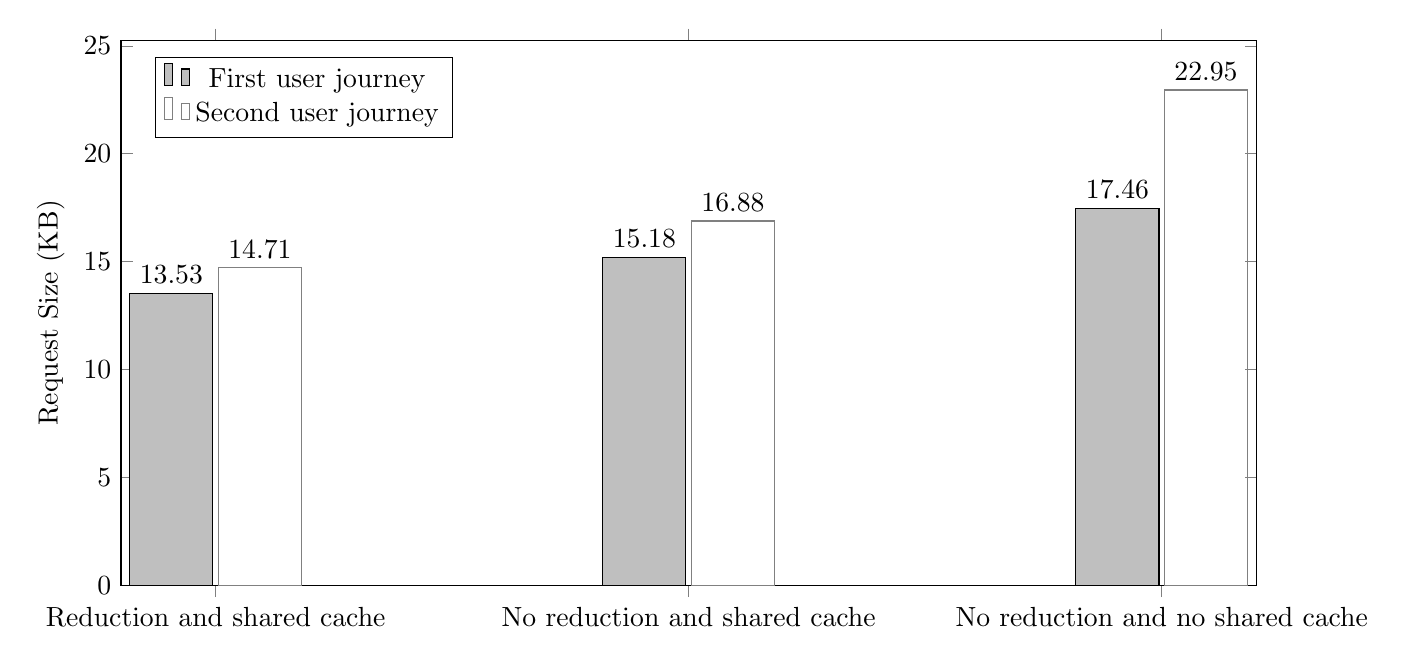
\begin{tikzpicture}
    \begin{axis}[
      ymin=0,
      ybar,
      legend pos=north west,
      ylabel={Request Size (KB)},
      xtick=data, 
      symbolic x coords={Reduction and shared cache, No reduction and shared cache, No reduction and no shared cache}, 
      nodes near coords align={vertical},
      nodes near coords,
      height=8.5cm,
      width=16cm,
      bar width=30pt,
      cycle list={
        {fill=lightgray, draw=gray}
      },
    ]
    \addplot coordinates {(Reduction and shared cache, 13.53) (No reduction and shared cache, 15.18) (No reduction and no shared cache, 17.46)};
    \addplot coordinates {(Reduction and shared cache, 14.71) (No reduction and shared cache, 16.88) (No reduction and no shared cache, 22.95)};
    \legend{First user journey, Second user journey}
    \end{axis}
  \end{tikzpicture}
  \caption{Request size comparison between the three approaches.}\label{fig:discussion:request-size}
\end{figure}

\noindent The next section compares the response sizes of the GraphQL \ac{API} of the three approaches.

\section{Response Size}\label{section:discussion:response-size}

This section compares the response sizes from the GraphQL \ac{API} of the three approaches. Figure \ref{fig:discussion:response-size} displays the results already shown in the previous sections \ref{section:results:comparison-first-journey} and \ref{section:results:comparison-second-journey} as a bar chart for better comparability. Clearly, visible is that the differences in response size are more significant than the difference in request size. As displayed in the figure, the difference between the approach with no query reduction and no shared cache is about 2.35 MB. Therefore, the 11 requests that are committed by using the shared caching are responsible for more than 2 MB of data that needs to be downloaded unnecessarily. This difference could make a huge difference in page performance when using a mobile device. The difference between the first and second approaches is only about 62 KB, which is not very significant and does not make a real difference. Saving 62 KB of data in 37 GraphQL queries is not worth the effort of implementing and using the query reduction. 

\bigskip

\noindent The second user journey shows a quite similar outcome, as the size differences are quite similar. The second approach in the second user journey omits 25 requests in comparison to the naive third approach. This results again in a difference of about 2.35 MB. There is just a 3 KB difference in response sizes between the first and second approaches. These differences are coming from the omitted fields from queries, which is quite small compared to the 37 GraphQL queries that are executed against the \ac{BFF}.

\bigskip

\noindent Just like with the request sizes, the query reduction does not make a significant improvement by reducing the size of the responses in comparison to just using the shared caching layer.

\begin{figure}[H]
  \centering
  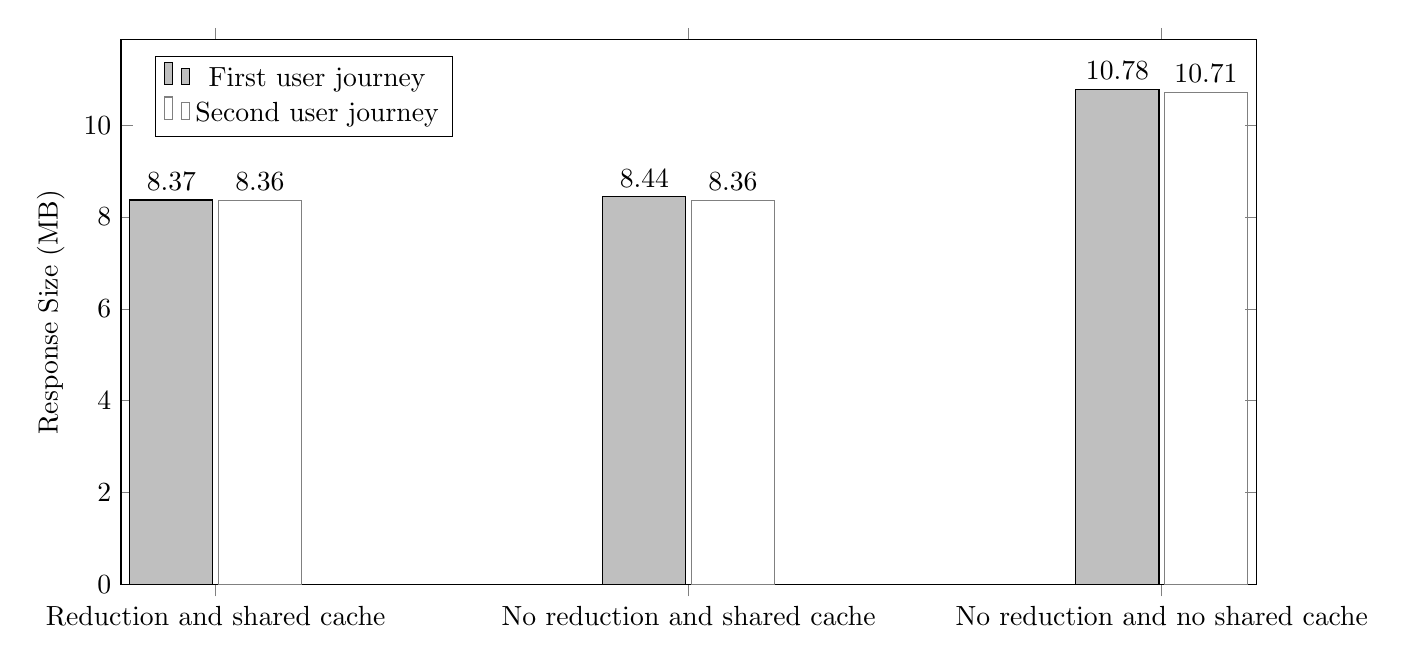
\begin{tikzpicture}
    \begin{axis}[
      ymin=0,
      ybar,
      legend pos=north west,
      ylabel={Response Size (MB)},
      xtick=data, 
      symbolic x coords={Reduction and shared cache, No reduction and shared cache, No reduction and no shared cache}, 
      nodes near coords align={vertical},
      nodes near coords,
      height=8.5cm,
      width=16cm,
      bar width=30pt,
      cycle list={
        {fill=lightgray, draw=gray}
      },
    ]
    \addplot coordinates {(Reduction and shared cache, 8.37) (No reduction and shared cache, 8.44) (No reduction and no shared cache, 10.78)};
    \addplot coordinates {(Reduction and shared cache, 8.361) (No reduction and shared cache, 8.364) (No reduction and no shared cache, 10.71)};
    \legend{First user journey, Second user journey}
    \end{axis}
  \end{tikzpicture}
  \caption{Response size comparison between the three approaches.}\label{fig:discussion:response-size}
\end{figure}

\noindent The next section takes the response into perspectives and compares the response times of the three approaches. This is important because smaller responses lead to faster responses, which is a crucial factor for the user experience.

\section{Response Times}\label{section:discussion:response-times}

It is hard to make real comparisons when it comes to measuring the time it takes to fetch the responses from the backend. The network speed can vary greatly over time, therefore it is not easy to make a reproducible comparison. Therefore, the measurement was done using the throttle mode inside the \href{https://developer.chrome.com/docs/devtools/}{Google DevTools}. The network speed was set to 1.5 Mbps also named \enquote{fast 3G} preset inside the developer tools. This ensures that the network speed stayed the same for all three approaches. The response times were measured three times for every approach and the mean value was taken to get a neutral value. The preset \enquote{fast 3G} was chosen because it is quite slow and makes it possible for times to differ more significantly. With faster network speeds, the differences would be smaller and harder to compare in general. And 3G is still a quite common network speed for mobile connections in many countries. 

\bigskip

\noindent This section measures the total time to download every query response from the GraphQL \ac{API} for the three approaches from section \ref{section:results:performance-measurement}. The measurement must not be misunderstood, because the browser loads the resources partially in parallel. Here only total download time is measured to see how much time is needed to download all the resources in one of the approaches. The measurements were recorded during the user journeys from section \ref{section:results:comparison-first-journey} and \ref{section:results:comparison-second-journey} alongside the request sizes and response sizes. Therefore the total response times correspond to the measured network sizes from the previous two chapters. The results are measured in seconds and are shown in figure \ref{fig:discussion:response-times}. The speeds

\begin{figure}[H]
  \centering
  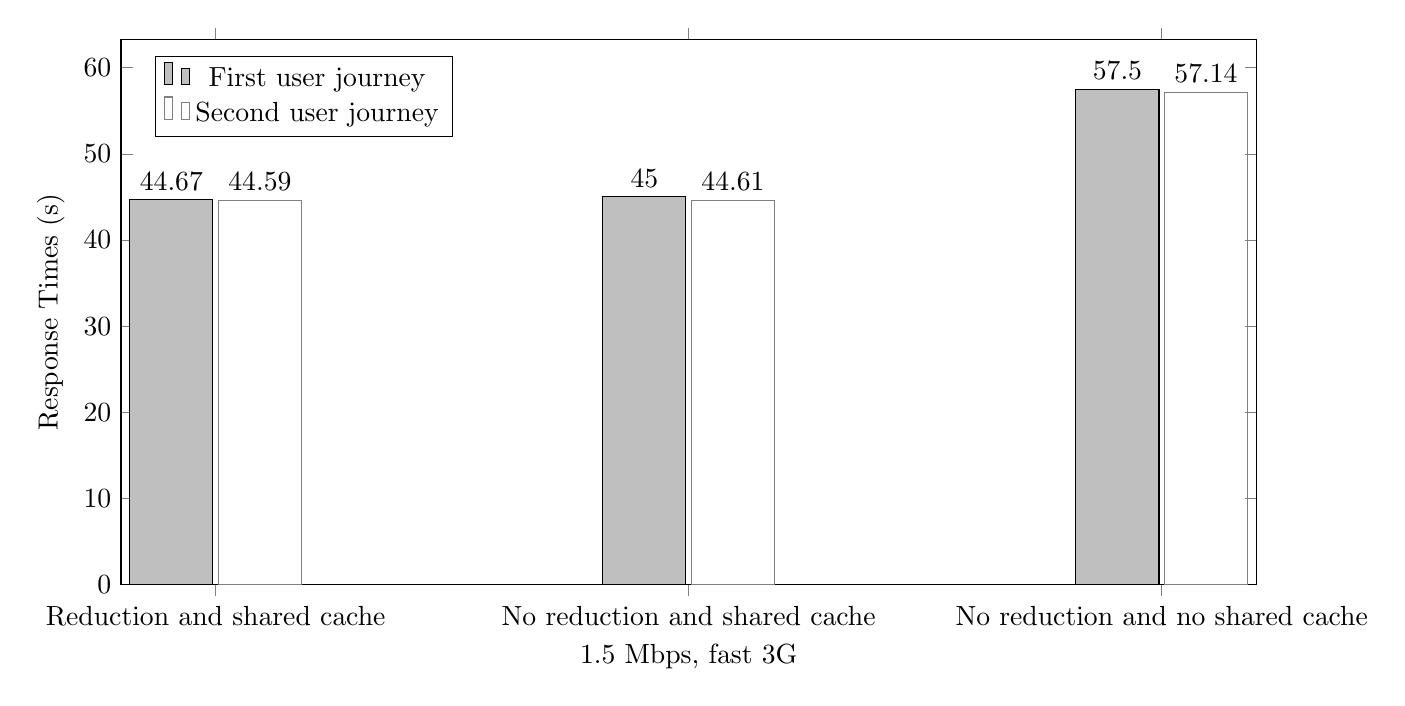
\begin{tikzpicture}
    \begin{axis}[
      ymin=0,
      ybar,
      legend pos=north west,
      ylabel={Response Times (s)},
      xlabel={1.5 Mbps, fast 3G},
      xtick=data, 
      symbolic x coords={Reduction and shared cache, No reduction and shared cache, No reduction and no shared cache}, 
      nodes near coords align={vertical},
      nodes near coords,
      height=8.5cm,
      width=16cm,
      bar width=30pt,
      cycle list={
        {fill=lightgray, draw=gray}
      },
    ]
    \addplot coordinates {(Reduction and shared cache, 44.67) (No reduction and shared cache, 45.00) (No reduction and no shared cache, 57.50)};
    \addplot coordinates {(Reduction and shared cache, 44.59) (No reduction and shared cache, 44.61) (No reduction and no shared cache, 57.14)};
    \legend{First user journey, Second user journey}
  \end{axis}
  \end{tikzpicture}
  \caption{Response time comparison between the three approaches.}\label{fig:discussion:response-times}
\end{figure}

\noindent Like before, the difference between the second approach and the third approach is quite significant. The second approach for both journeys is about 12 seconds faster than the third approach. The eleven respectively 25 requests that are omitted by using the shared caching layer are responsible for about 12 seconds of extra download time. The results from this measurement correspond to the response size measurement from the previous section \ref{section:discussion:response-size}. The results for both the first approach and the second approach are practically the same. The reduction of 37 queries does not yield the expected results and does not speak in favor of using query reduction.
\fi

\ifshowConclusionChapter
  \chapter{Conclusion}\label{chapter:conclusion}

\noindent To validate the first hypothesis, which states that using GraphQL with a common caching layer can prevent over-fetching and over-requesting, a micro-frontend architecture with 12 different applications was designed and implemented. In the future, it is planned to integrate the prototype with AGnet's micro-frontend architecture. Therefore, the GraphQL queries used will be used later in the real application and the results of the evaluations are very expressive.

\noindent First, the shared caching layer was implemented, and to further improve performance, a mechanism was written to reduce queries with content already in the cache.

\noindent Based on the groundwork three different approaches were identified, how the prototype could be evaluated. Just sharing the cache between the micro-frontends resulted in a total save 22\% of response-size in comparison to a separated cache.

\noindent But the reduction in queries doesn't make that much difference with the queries in this prototype. The difference in request-size is only a few kilobytes, and the difference in response-size is not large enough to make a real difference.

\noindent To validate the second hypothesis, which states that the prototype should provide enough freedom in the choice of technology, a micro frontend was written using React and embedded in the shell application. The application was able to integrate with the existing architecture and use both the shared caching layer and the query reduction mechanism. The architecture is thus open to the free choice of technology.

\fi

\ifshowFutureWorkChapter
  \chapter{Future work}\label{chapter:future-work}

\section{Another solution}

% \lipsum[1-5]

\section{Technology agnostic}

% \lipsum[1-5]

% examine a project that might improve from using query reduction

% the dashboard problems

% make the shell application and the communcation really technology agnostic

% The dashboard functionality of the approach is not well suited for the query reduction approach. But a use case, where the query reduction shines might be an e-commerce application like Amazon.
\fi


%
% Hier beginnen die Verzeichnisse.
%
\clearpage
\printbibliography
\clearpage

% Das Abbildungsverzeichnis
\listoffigures
\clearpage

% Das Tabellenverzeichnis
\listoftables
\clearpage

% Das Quellcodeverzeichnis
\listoflistings
\clearpage

\phantomsection
\addcontentsline{toc}{chapter}{\listacroname}

\chapter*{\listacroname}
\begin{acronym}[XXXXX]
    \acro{HTTP}{Hypertext Transfer Protocol}
    \acro{URL}{Uniform Resource Locator}
    \acro{API}{Application Programming Interface}
    \acro{SPA}{Single-Page-Application}
    \acro{BFF}{Backend For Frontend}
    \acro{REST}{Representational State Transfer}
    \acro{IP}{Internet-Procotol}
    \acro{HTML}{Hypertext Markup Language}
    \acro{IDE}{Integrated development environment}
    \acro{JSON}{JavaScript Object Notation}
    \acro{SQL}{Structured Query Language}
    \acro{GRPC}{gRPC Remote Procedure Calls}
    \acro{JS}{JavaScript}
    \acro{TS}{TypeScript}
    \acro{DI}{Dependency Injection}
    \acro{UI}{User Interface}
    \acro{ID}{Identifier}
    \acro{UML}{Unified Modeling Language}
\end{acronym}

%
% Hier beginnt der Anhang.
%
\clearpage
\appendix
\chapter{Anhang A}
\clearpage
\chapter{Anhang B}
\end{document}
